\documentclass[fontsize=10pt,openright,oneside,paper=a4,BCOR=1cm,numbers=noenddot]{scrbook}


\usepackage[top=3.5cm, bottom=3.5cm, left=3.0cm, right=4.0cm]{geometry}
\usepackage{lipsum}


%%%%%%%%%%%%%%%%%%%%%%%%%%%%%%%%%%%%%%%%%%%%%%%%%%%%%%%%%%%%
% Basic definitions, to be adjusted individually
\newcommand{\authornamefirst}{Eva}
\newcommand{\authornamelast}{Gründinger}
\newcommand{\matrikelnummer}{85500}
\newcommand{\authorhomestreet}{Bärnbach 6}
\newcommand{\authorpostalcodecity}{94116 Hutthurm}

\newcommand{\worktitle}{The IoT Security Pattern Landscape: Collection and Analysis of state-of-the-art Security Patterns for IoT Development}

\newcommand{\thesistype}{Master's Thesis}
% \newcommand{\thesistype}{Bachelor's Thesis}
\newcommand{\courseofstudies}{Computer Science}

\newcommand{\thesisdate}{2023-03-22}   %% in ISO 8601 format

\newcommand{\thesisprof}{Prof. Dr. Stefan Katzenbeisser}
\newcommand{\thesisproftwo}{Prof. Dr. Joachim Posegga}
\newcommand{\chair}{\mbox{Chair of Computer Engineering}}
\newcommand{\secondchair}{Chair of IT Security}

\newcommand{\advisor}{Felix Klement}


\newcommand{\contactprofone}{
\thesisprof \\
\chair \\
University of Passau \\
Email:~{\small \url{stefan.katzenbeisser@uni-passau.de}}  \\
Web:~{\small
\url{https://www.fim.uni-passau.de/en/computer-engineering}}\\}


\newcommand{\contactproftwo}{
\thesisproftwo \\
\secondchair \\
University of Passau \\
Email:~{\small \url{Joachim.Posegga@uni-passau.de}}  \\
Web:~{\small
\url{https://www.sec.uni-passau.de/en}}\\}


%\newcommand{\drosera}{\textit{Drosera}\xspace}
%%%%%%%%%%%%%%%%%%%%%%%%%%%%%%%%%%%%%%%%%%%%%%%%%%%%%%%%%%%%

% PACKAGES:

\usepackage{color}
\usepackage[colorinlistoftodos,prependcaption]{todonotes}
\usepackage{xargs}

\newcommandx{\mytodo}[2][1=]{\todo[linecolor=yellow,backgroundcolor=yellow!25,bordercolor=yellow,inline,#1]{#2}}

% Use English :

% Use list of tabels, etc. in table of contents:
\usepackage[nottoc]{tocbibind}
% German paragraph skip
\usepackage{parskip}
% Encoding. Use utf8. We are now in the 21st century already... :-)
\usepackage[utf8]{inputenc}
% Index-generation
\usepackage{makeidx}
% Einbinden von URLs:
\usepackage{url}
% Special \LaTex symbols (e.g. \BibTeX):
\usepackage{doc}
% Include Graphic-files:
%\usepackage{graphics}
% Include Graphic-files:
\usepackage{graphicx}
% Include doc++ generated tex-files:
%\usepackage{docxx}
% Include PDF links
\usepackage{listings}
\usepackage{float}
\usepackage{pgfplots}
\usepackage{multirow}
%mathstuff
\usepackage[cmex10]{amsmath}
\usepackage{amsfonts}
\usepackage{amssymb}
\usepackage{lscape}
\usepackage{longtable}
\usepackage{pgf-pie}
\usepackage{subfigure} 
\usepackage{pifont}% http://ctan.org/pkg/pifont
\newcommand{\cmark}{\ding{51}}%
\newcommand{\xmark}{\ding{55}}%
\usepackage{pdfpages}
\usepackage{multicol}
\usepackage{xspace}
\newcounter{mtpage}
\newcommand{\q}[1]{``#1''}

%hyperref for nice PDF output
\usepackage[pdftex, 
bookmarks=true,
pdfauthor={{{\authornamefirst \authornamelast}}},
pdftitle={{{\worktitle}}},
hidelinks
]{hyperref}

%%%%%%%%%%%%%%%%%%%%%%%%%%%%%%%%%%%%%%%%%%%%%%%%%%%%%%%%%%%%

% OTHER SETTINGS:

% Pagestyle:
\pagestyle{headings}

% Avoid 'overhang':
\sloppy

% Choose language
\newcommand{\setlang}[1]{\selectlanguage{#1}\nonfrenchspacing}

\usepackage[english]{babel}

\setlang{english}
%\setlang{german}

\usepackage[Bjornstrup]{fncychap}

\definecolor{bblue}{HTML}{00A2FF}
\definecolor{rred}{HTML}{FF2600}
\definecolor{ggreen}{HTML}{61D836}
\definecolor{ppurple}{HTML}{C24885}
\definecolor{oorange}{HTML}{F8BA00}
\definecolor{ggray}{HTML}{5F5F5F}
\definecolor{ppink}{HTML}{e81cbf}
\definecolor{dkgreen}{rgb}{0,0.6,0}
\definecolor{gray}{rgb}{0.5,0.5,0.5}
\definecolor{mauve}{rgb}{0.58,0,0.82}

\lstset{frame=tb,
	language=Java,
	aboveskip=3mm,
	belowskip=3mm,
	showstringspaces=false,
	columns=flexible,
	basicstyle={\small\ttfamily},
	numbers=none,
	numberstyle=\tiny\color{gray},
	keywordstyle=\color{blue},
	commentstyle=\color{dkgreen},
	stringstyle=\color{mauve},
	breaklines=true,
	breakatwhitespace=true,
	tabsize=3
}


%%%%%%%%%%%%%%%%%%%%%%%%%%%%%%%%%%%%%%%%%%%%%%%%%%%%%%%%%%%%

% TITLE:

\begin{document}
\frontmatter
\thispagestyle{empty}
\newpage

\vspace{1cm}

\begin{center}
\begin{tabular}{lr}
\includegraphics[width=6.5cm]{img/logouni_en.png}
\end{tabular}

\vspace{3cm}
\Large University of Passau
\\
\Large Faculty of Computer Science and Mathematics
\\
\vspace{0.3cm}
\Large {\chair }
\\
\Large \thesisprof

\end{center}


\vspace{2.5cm}

\begin{center}
        % Master's thesis, Bachelor's thesis, Programming project
        {\Large \thesistype\\ in \\ \courseofstudies} 
\end{center}

\begin{center}
        \settowidth{\baselineskip}{0.4cm}
        {\LARGE \textbf{\worktitle}}
        \\
        {\Large
        \vspace{1cm}
        \authornamefirst~\authornamelast \\ \matrikelnummer \\
        }
\end{center}

\vfill {% \settowidth{\baselineskip}{0.2cm}

\vfill


{\large
\begin{tabular}[l]{llll}

Date:       & \thesisdate %%(\LaTeX{}$2_\epsilon$ run \today)
\smallskip \\
Supervisors:   & \thesisprof \\
	& \thesisproftwo \\
Advisor: & \advisor \\
\end{tabular}}
} \cleardoublepage
%%%%%%%%%%%%%%%%%%%%%%%%%%%%%%%%%%%%%%%%%%%%%%%%%%%%%%%%%%%%


\include{legals}

% MAIN PART:

% Abstract. 
% !TeX spellcheck = en_GB
% !TeX encoding = UTF-8
% !TeX root = ../thesis.tex
\chapter*{Abstract}




% Table of contents
\tableofcontents

% Main body of thesis
\mainmatter
% !TeX encoding = UTF-8
% !TeX spellcheck = en_GB
% !TeX root = ../thesis.tex


\chapter{Introduction}\label{ch:introduction}
Today most smart devices are highly connected in a network that allows them to interact with each other. But this level of connectivity makes it difficult even for experts to keep the overview. These intelligent networks can be quite confusing when one does not have knowledge of the right tools/frameworks or when the needed technology does not even exist, yet. Many users also don't realize how dependent one can be on these devices and what security risks a connected world can bring. The first Section~\ref{sec:def} introduces the term Internet of Things (IoT) and follows up in Section~\ref{sec:areas} with different areas of life that these technologies are likely to be found in to get familiar with IoT for the following analysis.


\section{Definition of Internet of Things}\label{sec:def}
The term IoT itself is common knowledge and these \emph{\q{things}} are well-established in our society but only a few people know what exactly the \emph{\q{Internet of Things}} is. In this section we define which devices belong to IoT and in which areas of life IoT enhances the daily routines of people.
\begin{quote}
	\emph{\q{The Internet of Things (IoT) describes the network of physical objects — things — that are embedded with sensors, software, and other technologies for the purpose of connecting and exchanging data with other devices and systems over the internet.\footnote{\href{https://www.oracle.com/in/internet-of-things/what-is-iot}{https://www.oracle.com/in/internet-of-things/what-is-iot, last accessed: 12.10.2022.}}}}
\end{quote}
Although this quote from the oracle website gives a good general definition of what IoT encompasses, it is easier to understand the idea of IoT with an example: Picture a smart home in which every gadget and appliance inside the house is connected to the internet and communicates with each other. Using your smartphone one can lock the door and get notifications if an unauthorized person enters the backyard when he is detected by the installed motion sensors. The room temperature is regulated automatically with temperature sensors that are located outside and lights are controlled according to the time of day to save energy. More common examples and different types of IoT devices are:\footnote{\href{https://learn.g2.com/iot-devices}{https://learn.g2.com/iot-devices, last accessed: 21.10.2022.}}
\begin{itemize}
	\item Home security: Motion detection, automatic recording, remote arm or disarm
	\item Industrial IoT: Security or safety systems, machine sensors, project management
	\item Healthcare and fitness: Wearable healthcare devices, activity trackers
	\item Banking and financial services: ATMs, interactive payment cards
	\item Virtual/Augmented reality: Mobile or head-mounted AR, standalone VR
\end{itemize}
But the high connectivity and continuous data exchange between devices and applications has both benefits as well as disadvantages. 

\begin{itemize}
	\item[+] Time savings. By automating activities, it saves the user a lot of time.
	\item[+] Enhanced data collection. Information is easily accessible and frequently updated in real time.
	\item[+] Safety concerns. Devices sense potential danger and warn users in time. 
\end{itemize}

\begin{itemize}
	\item[--] Security issues. Hackers may gain access to the system and steal personal information.
	\item[--] High internet dependence. Devices are unable to function effectively without the internet.
	\item[--] Complexity. There are many risks of failure in IoT devices.
\end{itemize}


\section{Application Areas}\label{sec:areas}
After we discussed what IoT is in general and which devices belong to the IoT spectrum, we look into the application areas of this technology. Therefore we divide the field of IoT into five groups\footnote{\href{https://syntegra.net/internet-of-things-the-five-types-of-iot}{https://syntegra.net/internet-of-things-the-five-types-of-iot, last accessed: 12.10.2022.}} and explore the different ways IoT can be utilized.

\paragraph{Consumer Internet of Things (CIoT).}
All kinds of appliances, gadgets and other connected devices that are meant for user consumption are a part of CIoT. Typical products include smartphones, wearables, home appliances, etc. These are in most cases connected via Wi-Fi or Bluetooth for short-range communication inside the home. 

\paragraph{Commercial Internet of Things.}
Most Commercial IoT focuses on large venues in order to improve customer experience and business conditions. As an example these IoT devices can monitor environmental conditions, manage access control systems or economize utilities in office buildings, stores, healthcare institutions, entertainment venues or hotels.

\paragraph{Industrial Internet of Things (IIoT).}
In order to improve productivity and efficiency, most large-scale factories or manufacturing plants utilize IoT systems. IIoT can also be often found in the fields of healthcare, automotive, logistics, and agriculture. 

\paragraph{Infrastructure Internet of Things.}
For the development of smart infrastructures this type of IoT tries to design IoT systems that are able to increase efficiency while decreasing its costs. These IoT infrastructures are then used in monitoring and controlling operations that deal with public infrastructures like bridges, railway tracks or even windfarms.

\paragraph{Internet of Military Things (IoMT).}
Like its name suggests, IoMT or also called Internet of Battlefield Things (IoBT) is an important part of the modern military. By interconnecting ships, planes, tanks, soldiers and even drones on the battlefield, not only the situational awareness during war, but also risk assessments and response times can be greatly improved. The data that is collected during monitoring can then be utilized to enhance the IoT systems, equipment, military practices and strategies. 

% !TeX encoding = UTF-8
% !TeX spellcheck = en_GB
% !TeX root = ../thesis.tex

\chapter{Background}\label{ch:background}
In order to simplify the following argumentation in this master's thesis and amplify the importance of secure IoT design, Section~\ref{sec:iot-risks} describes common security risks that users of IoT devices should be aware of. Then we introduce the top ten IoT vulnerabilities according to OWASP (see Section~\ref{sec:owasp}) and lastly conclude this chapter with different design methods for secure IoT development in Section~\ref{sec:design}. 


\section{IoT Security Risks}\label{sec:iot-risks}
When looking back at the smart home example of Section~\ref{sec:def}, we realize how many connections between different IoT devices and appliances are needed as basis for a modern smart system. But each of these communication paths can be seen as a potential risk for a cyber attack and these interfaces are not the only vulnerabilities of an IoT device. Hackers constantly develop new techniques to gain access to and control IoT systems with millions of attacks occurring every day. To give a few examples of what typical cyber attacks on IoT devices are, here are ten types that attackers commonly use:\footnote{\href{https://micro.ai/blog/10-types-of-cyber-security-attacks-in-the-iot}{https://micro.ai/blog/10-types-of-cyber-security-attacks-in-the-iot, last accessed: 06.12.2022.}} 
\begin{itemize}
	\item Physical Attacks. After gaining access a USB drive is used to spread malicious code.
	\item Encryption Attacks. Capture of unencrypted data and control of system after decrypting the encryption keys.
	\item Denial of Service. One target is attacked by a larger number of systems which leads to services being unavailable.
	\item Firmware Hijacking. When firmware is not updated regularly, attackers can hijack it and download malicious software.
	\item Botnets. Usage of smart devices to transfer private corporate data or disable devices.
	\item Man-in-the-Middle. Intercepting the communication between two parties.
	\item Ransomware. By locking down files, this malware is used to blackmail corporations to pay money in order to get access to their data.
	\item Eavesdropping. Network traffic on a weak connection can be intercepted by an attack in order to gain sensitive data.
	\item Privilege Escalation. Hackers use user profiles with higher privileges to deploy malware and steal confidential data that otherwise would be impossible.
	\item Brute Force Password Attack. Also known as dictionary attack, the attacker tries a huge set of random phrases to access a password-protected service. 
\end{itemize} 


\section{Top Ten Common IoT Vulnerabilities}\label{sec:owasp}
What are the biggest problems when building and managing an IoT system? This question is analysed and periodically updated by the Open Web Application Security Project or in short: OWASP\footnote{\href{https://owasp.org}{https://owasp.org, last accessed: 13.10.2022.}}. The goal of this particular project is to help developers as well as users of IoT to better understand its security risks and give suggestions on how to make better decisions when working with this technology. Table~\ref{tab:owasp10} shows the top ten common IoT vulnerabilities from the year 2018 when OWASP last updated their results.\footnote{\href{https://wiki.owasp.org/index.php/OWASP_Internet_of_Things_Project}{https://wiki.owasp.org/index.php/OWASP\_Internet\_of\_Things\_Project, last accessed: 09.09.2022.}}

\begin{longtable}[c]{lp{4.5cm}p{7.5cm}}
	\caption{Internet of Things Top Ten (2018) taken from OWASP Wiki\protect\footnotemark[\value{footnote}]}
	\label{tab:owasp10}\\
	\hline
	\textbf{No.} & \textbf{Security Issue} & \textbf{Description} \\
	\hline
	\endfirsthead
	%
	\multicolumn{3}{c}%
	{{\bfseries Table \thetable\ continued from previous page}} \\
	\endhead
	%
	T1 & Weak, Guessable, or Hardcoded Password & Use of easily bruteforced, publicly available, or unchangeable credentials, including backdoors in firmware or client software that grants unauthorized access to deployed systems. \\
	T2 & Insecure Network Services & Unneeded or insecure network services running on the device itself, especially those exposed to the internet, that compromise the confidentiality, integrity/authenticity, or availability of information or allow unauthorized remote control.\\
	T3 & Insecure Ecosystem Interfaces & Insecure web, backend API, cloud, or mobile interfaces in the ecosystem outside of the device that allows compromise of the device or its related components. Common issues include a lack of authentication/authorization, lacking or weak encryption, and a lack of input and output filtering. \\
	T4 & Lack of Secure Update Mechanism & Lack of ability to securely update the device. This includes lack of firmware validation on device, lack of secure delivery (un-encrypted in transit), lack of anti-rollback mechanisms, and lack of notifications of security changes due to updates.\\
	T5 & Use of Insecure or Outdated Components & Use of deprecated or insecure software components/libraries that could allow the device to be compromised. This includes insecure customization of operating system platforms, and the use of third-party software or hardware components from a compromised supply chain.\\
	T6 & Insufficient Privacy Protection & User’s personal information stored on the device or in the ecosystem that is used insecurely, improperly, or without permission.\\
	T7 & Insecure Data Transfer and Storage & Lack of encryption or access control of sensitive data anywhere within the ecosystem, including at rest, in transit, or during processing.\\
	T8 & Lack of Device Management & Lack of security support on devices deployed in production, including asset management, update management, secure decommissioning, systems monitoring, and response capabilities.\\
	T9 & Insecure Default Settings & Devices or systems shipped with insecure default settings or lack the ability to make the system more secure by restricting operators from modifying configurations.\\
	T10 & Lack of Physical Hardening & Lack of physical hardening measures, allowing potential attackers to gain sensitive information that can help in a future remote attack or take local control of the device.\\
	\hline
\end{longtable}


\section{Secure IoT Design}\label{sec:design}
This section focuses on different methods software developers use to simplify programming practices for object-oriented systems. We will discuss relevant patterns and architectures that support the design of secure IoT systems, e.g. design patterns, security-specific patterns, and architectures.

\subsection{Design Patterns}
The concept of design patterns in software development can be traced back to 1994 and the \q{Design Patterns - Elements of Reusable Object-Oriented Software} book~\cite{Gamma1994}. The authors stated that a design pattern should be based on the following two principles:
\begin{itemize}
	\item Program to an interface not an implementation.
	\item Favour object composition over inheritance.
\end{itemize}
In general, design patterns are specific to a scenario and provide a standard terminology that help professionals in creating best solutions for certain common problems in their field. According to the referenced book, design patterns can be grouped into four different categories: 
\begin{itemize}
	\item Creational Patterns. Provide a way to create objects while hiding the creation logic.
	\item Structural Patterns. Inheritance is used to create interfaces and define ways to compose objects to obtain new functionalities.
	\item Behavioural Patterns. Manage communication between objects.
	\item J2EE Patterns. Concerned with the presentation tier (identified by Sun Java Center).
\end{itemize}
Related categories that should be mentioned in this context would be anti-patterns\footnote{\href{https://www.bmc.com/blogs/anti-patterns-vs-patterns}{https://www.bmc.com/blogs/anti-patterns-vs-patterns, last accessed: 17.10.2022.}} and misuse patterns~\cite{Fernandez2009}. These patterns focus on common development mistakes and attacks respectively but because of their specific usage they are not further relevant for the topic of this master's thesis.

\subsection{Security Patterns}
If design patterns are re-usable solutions for common design problems, similar to that security patterns are intended to achieve specific security goals in a system. The security-by-design principle makes sure that the security aspect is in the forefront of the design process, integrated into the system and not added as an after-thought. The most important security goals are: \emph{Confidentiality, Integrity, Availability, Authentication, and Authorization}. A subcategory of security patterns can be found in the so-called privacy patterns\footnote{\href{https://privacypatterns.org}{https://privacypatterns.org, last accessed: 17.10.2022.}} that are specialized to guide developers in finding the best solution for common privacy problems in software development. They support developers in modelling privacy-by-design and creating practical software solutions in a standardized way.


\subsection{Security Architectures}
Cybersecurity threats are getting increasingly more common these days. As a way to protect ones system from cyberattacks and data breaches, security-specific architectures\footnote{\href{https://www.dig8ital.com/post/what-is-security-architecture-and-what-do-you-need-to-know}{https://www.dig8ital.com/post/what-is-security-architecture-and-what-do-you-need-to-know, last accessed: 19.10.2022.}} can be used. These architectures enable developers to implement their security goals and keep their digital assets safe by ultimately utilizing a set of security principles, methods and models. Every architect needs guidelines to work with. In the context of security architectures these rules are called \emph{frameworks}. There exist many international framework standards with The Open Group Architecture Framework (TOGAF), Sherwood Applied Business Security Architecture (SABSA) and Open Security Architecture (OSA) being common examples. Software breaches can mean very expensive losses for a company, not only in financial aspects but also the reputation of a company suffers. There are many good reasons to utilize a strong security architecture like:\footnotemark[\value{footnote}] 
\begin{itemize}
	\item Fewer security breaches. A strong security architecture is able to close common weaknesses and reduces the risk of successful system attacks. 
	\item Money savings. Proactive security measures are able to detect and fix vulnerabilities earlier in the product development cycle. The later an error is detected, the more money it can cost. 
	\item Disciplinary measures mitigation. In the event of an attack it matters to which degree the business tried to reduce its risk and prevent vulnerabilities beforehand in order to get a favourable outcome according to the regulations.
\end{itemize}

After establishing a definition for IoT, giving examples for common vulnerabilities in IoT systems and describing popular design methods in the context of IoT development, the basis for this master's thesis has been created. The following analysis will showcase the landscape of today's research in the field of IoT patterns and the lack of existing security-specific solutions. By collecting and sorting all gathered patterns into an exhaustive catalogue, a well-documented and hierarchically organized list was created that will guide future projects in the development of more security-focused systems.   


% !TeX encoding = UTF-8
% !TeX spellcheck = en_GB
% !TeX root = ../thesis.tex

\chapter{Related Work}\label{ch:related_work}
There are already many papers and articles that describe the relevance of patterns and architectures that focus specifically on IoT. But besides common design patterns and frameworks, security-specific patterns for IoT applications are still in their early stages of development and documentation and therefore rare to find. Here is a short excerpt to give an overview of important publications for the IoT development and to show the areas that are still lacking in research, e.g. IoT security patterns.


\section{General Patterns for IoT Design}
Design, privacy or security patterns are only a few examples of potential solutions to common development problems that IT experts face on a daily basis. The landscape of patterns and architectures that support the IoT market is huge and research can be found in many articles like the following.

\paragraph{Applying IoT Patterns to Smart Factory Systems.} Patterns are a common way to describe abstract solutions to design problems and can be used to analyse and understand computer systems in an easier way. Reinfurt et al.~\cite{Reinfurt2017} describe in their paper IoT-specific patterns that help to design IoT systems that can be applied to the domain of smart factory systems. These patterns cover different areas and operation modes like device communication and management as well as energy supply types.

\paragraph{IoT Architectural Styles.} Other than design patterns, different architecture styles can be utilized when creating IoT systems. Muccini et al.~\cite{Muccini2018} provide a number of abstract IoT reference architectures in their paper. By conducting a systematic mapping study a set of 63 papers was chosen out of over 2,300 potential works. The results of this study will help to classify existing and future approaches for IoT styles and patterns at the architectural level.

\paragraph{Landscape of Architecture and Design Patterns for IoT Systems.} In order to get a better idea for the landscape of patterns and architectures that have accumulated over the years in research, Washizaki et al.~\cite{Washizaki2019, Washizaki2020} analysed the successes and failures of used patterns for IoT systems. Because of limited documentation and a lack of successfully executed implementations, there is a lot of room for improvement in the development of IoT-specific patterns and architectures.  


\section{Security-specific IoT Patterns}
Unlike general frameworks that can be utilized by developers to simplify their work and help to solve problems on a more abstract level, domain-specific IoT patterns that also focus on security are difficult to find. Security objectives are a huge part of every computer system to protect the user's data and identity but, unfortunately, patterns that could prevent unauthorized access are lacking. There exist many ways an attacker can compromise IoT systems that are especially easy to exploit because of a vast variety of interfaces and connections that lead to vulnerabilities. 

\paragraph{Architectural Patterns for Secure IoT Orchestrations.} Fysarakis et al.~\cite{Fysarakis2019} sketch the SEMIoTICS approach to create a pattern-driven framework that is based on already existing IoT platforms. Aiming to guarantee secure actuation and semi-automatic behaviour, the SEMIoTICS project utilizes patterns to encode dependencies between security, privacy, dependability and interoperability properties of smart objects.

\paragraph{Towards a Collection of Security and Privacy Patterns.} Organized in an hierarchical taxonomy, Papoutsakis et al.~\cite{Papoutsakis2021} collect and categorize a set of security and privacy patterns. While giving the reader an overview of security- and privacy-related objectives that are relevant in the IoT domain, the goal of this paper is to match these properties to their corresponding patterns. This usable pattern collection should guide developers to create IoT solutions that are secure and privacy-aware by design.

\paragraph{A Decade of Research on Patterns and Architectures for IoT Security.} Over the last three years, Rajmohan et al.~\cite{Rajmohan2020, iotbds20, Rajmohan2022} published different papers that review the research work regarding IoT patterns and architectures for IoT security and privacy. Although there is a rise in number of publications, there is not yet an approach of applying architectures and patterns in a way that addresses security not only on the architectural but also on the network or IoT devices level. \\

Although the IoT research in academia is thriving and there exist a variety of design patterns, architectures and frameworks that can be utilized in the development of modern IoT devices, the lack of focus on security objectives is worrisome. Security patterns can not only guide developers to build safer systems but lessen the workload by taking already existing solutions for abstract problems. This master's thesis will make an important contribution in increasing the accessibility to these already existing IoT security patterns for future work in this field.  
% !TeX encoding = UTF-8
% !TeX spellcheck = en_GB
% !TeX root = ../thesis.tex

\chapter{Methodology}\label{ch:methodology}
This chapter introduces the research methodology and review protocol that is based on the systematic literature review (SLR) (in Section~\ref{sec:slr}) and used in order to search for the needed primary studies to answer the following research questions in Section~\ref{sec:research_questions}. The taxonomy that is needed to gather information from the collection of studies is then defined in Section~\ref{sec:taxonomy}.


\section{Systematic Literature Review}\label{sec:slr}
According to Kitchenham et al.~\cite{Kitchenham2007} SLR is an analysis of publications about a certain topic that collects and critically evaluates multiple research studies or papers in a systematic way. Its purpose is to provide an exhaustive summary of the available literature relevant to a specific research question in a transparent and reproducible way. The following points utilize the review protocol that is used to conduct the literature review in a strategic manner and consist of the research questions that should be answered, selection criteria the found papers need to fulfil and a search strategy on how to browse databases in order to find the most relevant publications.

\subsection{Research Questions}\label{sec:research_questions}
This thesis aims to answer the following research questions (RQs):

\begin{enumerate}
	\item[RQ1] Which layer in the IoT World Forum Reference Model is covered by the least security patterns?
	\item[RQ2] Which security goal is addressed by security patterns the least and how can the coverage be improved?
	\item[RQ3] How many of the OWASP top ten most common IoT vulnerabilities are solved by utilizing these security patterns?
\end{enumerate}

\subsection{Selection Criteria}
To minimize bias in the search and selection of our primary studies for this master's thesis, we predefined guidelines that need to be fulfilled for a study to be used in our analysis. This approach leads us to the following inclusion and exclusion criteria:

\subsubsection{Inclusion Criteria:}\label{subsubsec:ICs}
\begin{enumerate}
	\item[IC1] A primary study must contain (one or more) security pattern that is applicable to an IoT system.
	\item[IC2] A primary study must target the IoT field, either in a general or specific application domain of IoT.
	\item[IC3] A primary study must discuss security objectives for system design, architecture or infrastructure.
\end{enumerate}

\subsubsection{Exclusion Criteria:}\label{subsubsec:ECs}
\begin{enumerate}
	\item[EC1] Papers not written in the English language are filtered out.
	\item[EC2] Papers that discuss design, privacy or misuse patterns as well as security architectures for the IoT domain are excluded.
	\item[EC3] Papers that are not peer-reviewed are also ruled out. 
\end{enumerate}
 

\subsection{Search and Selection Strategy}
This section focuses on the selection of appropriate primary studies that can serve as a basis to answer the aforementioned research questions. The goal is to collect as many primary studies as possible that are relevant for this thesis. The strategy to find papers that discuss security patterns is divided into two main parts: automatic and manual search. First we let a set of search engines find example studies in an automated approach with specific keywords. Here we also apply the mentioned inclusion and exclusion criteria to exclude any unwanted results ahead of time. Second we conduct a manual search in order to fill the gaps with any relevant scientific papers that were missed by the machine. In an attempt to avoid duplicates, the last stage of the search process consists of merging identical papers that were found by different search engines. The exact procedure is described in the following points and illustrated in Figure~\ref{fig:search-overview}.

\subsubsection{1. Database search:} 
As our primary search engines, we utilized five well known databases for scientific publications: IEEE Xplore\footnote{\href{https://ieeexplore.ieee.org}{https://ieeexplore.ieee.org, last accessed: 21.05.2022.}}, ACM Digital Library\footnote{\href{https://dl.acm.org}{https://dl.acm.org, last accessed: 21.05.2022.}}, ScienceDirect\footnote{\href{https://www.sciencedirect.com}{https://www.sciencedirect.com, last accessed: 21.05.2022.}}, Web of Science\footnote{\href{https://access.clarivate.com}{https://access.clarivate.com, last accessed: 21.05.2022.}} and Scopus\footnote{\href{https://www.scopus.com}{https://www.scopus.com, last accessed: 21.05.2022.}}. Because Scopus and ACM Digital Library already reference SpringerLink\footnote{\href{https://link.springer.com}{https://link.springer.com, last accessed: 21.05.2022.}}, we could exclude the former as well as Researchgate\footnote{\href{https://www.researchgate.net}{https://www.researchgate.net, last accessed: 21.05.2022.}} and Google Scholar\footnote{\href{https://scholar.google.com}{https://scholar.google.com, last accessed: 21.05.2022.}} which also include many non-peer-reviewed and non-English papers. Based on Kitchenham et al.~\cite{Kitchenham2007} we created keywords that generate papers that are relevant for the answers to our research questions. This led us to the following search query that was used for our initial database search on May 21st, 2022: 
\begin{center}
	(\emph{\q{Internet of Things}} \textbf{OR} \emph{\q{IoT}} \textbf{OR}  \emph{\q{Cyber Physical Systems}} \textbf{OR} \emph{\q{Web of Things}}) \\ \textbf{AND} \\
	(\emph{\q{Security Pattern}} \textbf{OR} \emph{\q{Security Design Pattern}})	
\end{center}	
For each search the query string needed to be slightly modified to fit each database's advanced search functionality and guidelines.
	
\subsubsection{2. Manual search:} 
By utilizing the snowballing strategy that was introduced by Wholin and Prikladnicki~\cite{Wohlin2013}, we searched manually for further literature that was missed by the automatic database inquiry. Following references of the already found papers, we looked for relevant publications that include further security design patterns that can be useful for our study. After a few iterations we found a set of papers that met the inclusion criteria of our SLR. After eliminating any duplicates of papers that were already discovered by the initial database search, we could add eleven more articles to our database search result. By including these manual publication findings, our RQs can be answered in a more thorough way. 

\begin{figure}[ht]
	\includegraphics[scale=0.3]{img/search}
	\centering
	\caption{Overview of the search and selection procedure}
	\label{fig:search-overview}
\end{figure}


\section{Taxonomy of the Research Area}\label{sec:taxonomy}
In this section the taxonomy of IoT security patterns is introduced. The main purpose of the taxonomy classifications is to simplify the extraction and comparison of patterns that are described in the primary studies. Subsection~\ref{subsec:posa} defines a scheme on how to structure the pattern descriptions, then Subsection~\ref{subsec:model} depicts what the general architecture of an IoT system looks like and Subsection~\ref{subsec:security} shows which security goals are the main focus of the extracted patterns as the last part of the taxonomy classifications.

\subsection{Pattern Description with POSA}\label{subsec:posa}
All patterns in the catalogue will be listed utilizing the Pattern-Oriented Software Architecture (POSA) form, so that the descriptions of IoT security patterns in this master's thesis are presented in a unified form. Although POSA is a popular format, not all patterns in the analysed publications are presented in this way or do have a standardized format at all. Another very popular form is Gang of Four (GoF) which is used in the \q{Design Patterns: Elements of Reusable Object-Oriented Software} book~\cite{Gamma1994}. But we chose POSA because it is a well-accepted and widely used pattern description format that provides standard templates~\cite{Bunke2014} and is used in the book with the same name by Buschmann et al.~\cite{Buschmann1996}. Other pattern description formats can also be easily converted and mapped to the POSA form that describes design patterns with the following keywords: \emph{Intent, Example, Context, Problem, Structure, Solution, Dynamics, Consequences, Implementation, Example Resolved, Known Uses, and Related Patterns}. Because of space limitations and to structure the pattern catalogue in a concise and clear way, we reduced the used keywords to the most important ones which are \emph{Intent, Problem, and Solution}.

\subsection{IoT World Forum Reference Model}\label{subsec:model}
In order to keep our pattern catalogue organized, we utilize the IoT architecture of the IoT World Forum Reference Model\footnote{\href{https://www.m2mology.com/iot-transformation/iot-world-forum}{https://www.m2mology.com/iot-transformation/iot-world-forum, last accessed: 10.06.2022.}} (WFRM) for a layered hierarchy the found security patterns can be categorized in. This model is an attempt of the IoT World Forum to create a common model to guarantee interoperability between all IoT components. It is important to note that this model is not representative of a real IoT system but only an abstraction that was created in order to simplify IoT product development between vendors. A summary of each layer with its functionality is shown in Table~\ref{tab:IoT-world-ref}.

\paragraph{L1 Physical Devices \& Controllers.}
The outermost layer consists of the physical devices that are the \q{things} in the IoT architecture as well as the sensors and edge node devices connected to them. Almost any electronic device that has a network connection is either an IoT device or has one embedded. The most common types are:

\begin{itemize}
	\item \textbf{Sensors:} Optical sensors, temperature sensors,...
	\item \textbf{Security devices:} Security cameras, audio recording devices, motion sensors,...
	\item \textbf{Smart wearable devices:} Watches, earbuds, glasses,...
	\item \textbf{Intelligent appliances:} Smart thermostats, intelligent refrigerators, connected televisions,...
	\item \textbf{Actuators}
\end{itemize}

\paragraph{L2 Connectivity.}
The communication and processing unit has a wide range in the IoT model. From edge node devices to the cloud up to the next layer, Edge Computing, this layer is responsible for the information transport in the IoT network. Implementations vary from case to case with single to multiple technology solutions. Wired, wireless or cellular as well as multi-tiered architectures are just a few alternatives, that can be used alongside Field Area Networks, that are suitable for a mix of private and public package transport.

\paragraph{L3 Edge Computing.}
The previously mentioned Edge Computing layer is also called \q{Cloud Edge} or \q{Cloud Gateway} computing. Its purpose is to interface the data and control levels to the higher cloud, SaaS or enterprises layers and therefore makes this layer essential in any IoT architecture model. This layer is not only able to route to software functions and convert protocols but also to execute logic to reduce the decision making time and decrease latencies in the execution phase.

\paragraph{L4 Data Accumulation.}
For an efficient data stream there need to be storages that are responsible for queues between different architecture layers. Velocity, volume and variety should be continuously provided for incoming data in an IoT system. In order to be able to process and prepare the input stream for delivery to the next stage, this layer is implemented as an intermediate storage facility in the IoT WFRM. From simple solutions like the usage of SQL to more advanced distributed storage and processing systems like Hadoop and Hadoop File System, Mongo, Cassandra, Spark or other NoSQL versions, each IoT system has its own data management architecture.

\paragraph{L5 Data Abstraction.}
To get an overview of the incoming data, the Data Abstraction layer analyses and then organises information from different IoT devices, maps them into given schemata and prepares the extracted data for further upstream or downstream processing. For a simplified data flow the software frameworks for publish/subscribe or data distribution services are key elements. These architectures guarantee low latency high performance communication between Edge Computing, Data Accumulation, Applications and User Processes. 

\paragraph{L6 Application.}
Just as its name suggests, this layer is where all important application logic is executed. To just name a few, there are IoT related applications, user patterns, statistical analysis, alarm systems, logistical processes, monitoring and optimization techniques as examples that come to mind.

\paragraph{L7 Collaboration \& Processes.}
User interaction is the significant point in this layer of every IoT system. Data that was processed in lower layers is integrated into applications that are responsible for user engagement and economic value. The big challenge is to utilize IoT devices and its architecture model in such a way that it brings growth and value to the businesses and/or social good.

\begin{table}[ht]
	\centering
	\caption{Summary of IoT architecture layers\protect\footnotemark[\value{footnote}]}
	\label{tab:IoT-world-ref}
	\begin{tabular}{lll}
		\hline
		\textbf{No.} & \textbf{IoT Layer} & \textbf{Functionality} \\
		\hline
		L7 & Collaboration \& Processes & User Interaction, Business Processes \\
		L6 & Application & Reporting, Control, Analytics  \\
		L5 & Data Abstraction & Aggregation, Access \\
		L4 & Data Accumulation & Storage Facilities \\
		L3 & Edge Computing & Data Element Analysis, Transformation \\
		L2 & Connectivity & Message Transmission, Processing \\
		L1 & Physical Devices & The \q{Things} \\
		\hline 
	\end{tabular}
\end{table}

\subsection{Security Concerns}\label{subsec:security}
Each extracted IoT security pattern focuses on a specific security objective it tries to protect. The following paragraphs describe the most important security goals for IoT systems that should be covered by these security patterns for a secure software design. Hereby, the privacy goal is not further analysed in this master's thesis because of the exclusion criteria that were introduced in Subsection~\ref{subsubsec:ECs}. Specifically EC2 states that all papers that discuss privacy patterns are excluded from the analysis.

\paragraph{Confidentiality} is the objective to ensure that data resources or information are protected against unauthorized disclosure. Encryption and setting passwords are the most common measures to enforce this security objective.

\paragraph{Integrity} has the goal to protect data resources or information against unauthorized changes, tampering, destruction or loss. This security objective ensures that the data stays accurate and reliable.

\paragraph{Availability} means that data resources or information are accessible to authorized users. It provides an assurance that a system and its data can be accessed by authenticated users when they are needed.

\paragraph{Authentication} is the process of determining if an entity's identity is who he or she claims to be. Before a user can access stored information, he or she must prove their identity and permission to access the data.

\paragraph{Authorization} is the process of determining if a user has permission to access or use a certain resource. It is usually enforced in combination with authentication by access control mechanisms.

\paragraph{Privacy} is a subset of security that focuses on personal information. It describes the ability to protect sensitive data about personally identifiable information. 
% !TeX encoding = UTF-8
% !TeX spellcheck = en_GB
% !TeX root = ../thesis.tex

\chapter{IoT Security Pattern Catalogue}\label{ch:catalogue}
This chapter lists all IoT security patterns that were collected during the previously explained search process in form of a catalogue for IoT developers. The pattern table~\ref{tab:patterns} is divided into the seven layers of the World Forum Reference Model (WFRM). Each pattern corresponds to a specific layer and is described by its name, a list of vulnerabilities from the OWASP top ten it can (possibly) solve as well as security objectives that are either addressed by this particular pattern (+) or not mentioned in its original description (-).

For a more efficient use of space in the table that makes the information more concise but still easy to understand, we used specific abbreviations. Most of them were already previously introduced in this master's thesis. For a compact overview of the defined abbreviations, the following Table~\ref{tab:key} can be utilized.

\begin{longtable}[c]{|cl|cl|}
	\caption{Legend for pattern lookup table}
	\label{tab:key}\\
	\hline
	\multicolumn{2}{|c|}{\textbf{WFRM Architecture Layers}} & \multicolumn{2}{|c|}{\textbf{OWASP Top Ten Vulnerabilities}}\\
	\hline
	\endhead
	%
	L1 & Physical Devices \& Controllers & T1 & Weak, guessable or hardcoded passwords \\
	L2 & Connectivity & T2 & Insecure network services \\
	L3 & Edge Computing & T3 & Insecure ecosystem interfaces \\
	L4 & Data Accumulation & T4 & Lack of secure update mechanisms \\
	L5 & Data Abstraction & T5 & Use of insecure or outdated components \\ 
	L6 & Application & T6 & Insufficient privacy protection \\
	L7 & Collaboration \& Processes & T7 & Insecure data transfer and storage \\ 
	\cline{1-2}
	\multicolumn{2}{|c|}{\textbf{Security Objectives}} & T8 & Lack of device management\\
	\cline{1-2}
	C & Confidentiality & T9 & Insecure default settings  \\
	I & Integrity & T10 & Lack of physical hardening \\
	A & Availability & & \\
	Ac & Authentication & & \\
	Az & Authorization & & \\
	\hline 
\end{longtable}


\begin{landscape}
\begin{longtable}[c]{lllcccccccccccccccc}
	\caption{IoT security pattern lookup table}
	\label{tab:patterns} \\
	\hline
	\textbf{Layer} & \textbf{\#} & \textbf{Pattern Name} & \multicolumn{10}{c}{\textbf{Solution for}} & \multicolumn{5}{c}{\textbf{Security Concerns}} \\
	& & & T1 & T2 & T3 & T4 & T5 & T6 & T7 & T8 & T9 & T10 & C & I & A & Ac & Az \\
	\hline
	\endhead
	%
	\multirow{5}{*}{\textbf{L1}} & \ref{p:hardware} & Hardware IoT Security & & \checkmark & & \checkmark & \checkmark & & & & & & + & - & - & + & - \\
	& \ref{p:thing} & Secure IoT Thing & & \checkmark & \checkmark & & & & \checkmark & & & & + & + & + & - & - \\
	& \ref{p:node} & Secure Sensor Node & & & \checkmark & & \checkmark & & \checkmark & & & & + & + & + & + & + \\
	& \ref{p:segment} & Security Segmentation & & & \checkmark & & & & & & & & - & - & - & + & + \\
	& \ref{p:tpm} & Trusted Platform Module & & & & & \checkmark & & \checkmark & & & & + & + & - & + & + \\
	\hline
	%
	\multirow{14}{*}{\textbf{L2}} & \ref{p:ac} & Authenticated Channel & & \checkmark & & & & & \checkmark & & & & - & + & - & + & - \\ 
	& \ref{p:ec} & Encrypted Channel & & \checkmark & & & & & \checkmark & & & & + & - & - & - & - \\
	& \ref{p:broker} & Middleware Message Broker & & & \checkmark & & & & \checkmark & & & & + & - & - & - & - \\
	& \ref{p:scmessage} & Middleware Self-contained Message & & & & & & & \checkmark & & & & + & - & - & - & - \\
	& \ref{p:sdn} & Orchestration of SDN Network Elements & & & \checkmark & & & & \checkmark & & & & + & - & - & - & - \\
	& \ref{p:con} & Outbound-Only Connection & & & & & & \checkmark & \checkmark & & & & + & - & - & - & + \\
	& \ref{p:keyex} & Password Based Key Exchange & \checkmark & & & & & & \checkmark & & & & + & - & - & - & - \\
	& \ref{p:sc} & Safe Channel & & \checkmark & & & & & \checkmark & & & & - & + & - & - & - \\  
	& \ref{p:readout} & Secure Remote Readout & & & & & & & \checkmark & & & & + & + & - & + & - \\  
	& \ref{p:sm} & Signed Message & & & & & & & \checkmark & & & & - & + & - & + & - \\
	& \ref{p:crypto} & Symmetric Key Cryptography & & & & & & & \checkmark & & & & + & - & - & + & - \\
	& \ref{p:auc} & Third Party Based Authentication & & & & & & & \checkmark & & & & + & + & - & + & - \\
	& \ref{p:partner} & Trusted Communication Partner & & & & & & \checkmark & \checkmark & & & & + & - & + & + & + \\
	& \ref{p:trust} & Web of Trust & & & & & & & \checkmark & & & & - & + & - & + & - \\
	\hline
	%
	\multirow{3}{*}{\textbf{L3}} & \ref{p:fog} & Fog Computing & & \checkmark & \checkmark & & & & \checkmark & & & & + & + & + & + & + \\ 
	& \ref{p:fogxy} & Fogxy & & \checkmark & \checkmark & & & & \checkmark & & & & - & - & + & + & + \\ 
	& \ref{p:cloud} & Secure Cloud-based IoT Architecture & & & \checkmark & & & & \checkmark & & & & + & + & + & + & + \\
	\hline
	%
	\multirow{3}{*}{\textbf{L4}} & \ref{p:es} & Encrypted Storage & & & & & & \checkmark & \checkmark & & & & + & - & - & - & - \\
	& \ref{p:rs} & Redundant Storage & & & & & & & \checkmark & & & & - & - & + & - & - \\
	& \ref{p:ss} & Safe Storage & & & & & & \checkmark & \checkmark & & & & - & + & - & - & - \\
	\hline
	%
	\multirow{4}{*}{\textbf{L5}} & \ref{p:translation} & Alignment-based Translation Pattern & & & \checkmark & & & & & & & & - & - & + & - & - \\
	& \ref{p:block} & BlockBD & & & \checkmark & & & & \checkmark & & & & + & + & + & - & - \\
	& \ref{p:discover} & Discovery of IoT Services & & & \checkmark & & & & & & & & - & - & + & - & - \\
	& \ref{p:flow} & Flow-based Service Composition & & \checkmark & & & & & \checkmark & & & & + & - & - & - & - \\ 
	\hline
	\multirow{8}{*}{\textbf{L5}} & \ref{p:gateway} & IoT Gateway Event Subscription & & & \checkmark & & & & \checkmark & & & & + & - & + & - & - \\
	& \ref{p:ssl} & IoT SSL Cross-Layer Secure Access & & & \checkmark & & & & & & & & + & + & - & + & + \\
	& \ref{p:msgtranslator} & Middleware Message Translator & & & \checkmark & & & & & & & & - & - & + & - & - \\
	& \ref{p:middleware} & Middleware Simple Component & & & & & & & & & & & + & - & - & - & - \\
	& \ref{p:rest} & D2D REST Request/Response & & & \checkmark & & & & & & & & + & - & + & - & + \\
	& \ref{p:sandbox} & Server Sandbox & & & & & & & & & \checkmark & \checkmark & + & + & + & - & - \\ 
	& \ref{p:orchest} & Service Orchestration & & & \checkmark & & & & \checkmark & & & & + & - & - & - & - \\
	& \ref{p:ontology} & Translation with Central Ontology & & & \checkmark & & & & & & & & - & - & + & - & - \\
	\hline
	%
	\multirow{15}{*}{\textbf{L6}} & \ref{p:acp} & Access Control to Physical Structures & & & & & & & & & & \checkmark & - & - & - & + & + \\
	& \ref{p:alarm} & Alarm Monitoring & & & & & & & & \checkmark & & & - & - & - & - & + \\
	& \ref{p:log} & Audit Log & & & & & & & & \checkmark & & & - & + & - & - & - \\  
	& \ref{p:acs} & Authenticated Session & & & \checkmark & & & & & & & & - & - & - & + & - \\
	& \ref{p:aze} & Authorization Enforcer & & & & & & & & \checkmark & & & - & - & - & - & + \\
	& \ref{p:ep} & Encrypted Processing & & & & & & & \checkmark & & & & + & - & - & - & - \\
	& \ref{p:fault} & Fault Management & & & & & & & & \checkmark & & & - & - & + & - & - \\ 
	& \ref{p:fac} & File Authentication & & & & & & & \checkmark & & & & - & - & - & + & + \\
	& \ref{p:mac} & Matrix Authentication & & & & & & & \checkmark & & & & - & - & - & + & + \\
	& \ref{p:mine} & Minefield & & & & & \checkmark & & & & \checkmark & & - & + & - & - & - \\
	& \ref{p:rac} & Remote Authenticator/Authorizer & & & & & & & \checkmark & & & & - & - & - & + & + \\
	& \ref{p:rbac} & Role Based Access Control & & & & & & & \checkmark & & & & - & - & - & - & + \\
	& \ref{p:sp} & Safe Processing & & & & & & & \checkmark & & & & - & + & - & - & - \\
	& \ref{p:sdps} & Secure Distributed Publish/Subscribe & & & & & & & \checkmark & & & & + & + & + & + & + \\
	& \ref{p:uptime} & Uptime & & & & & & & & \checkmark & & & - & - & + & - & - \\
	\hline
	%
	\multirow{6}{*}{\textbf{L7}} & \ref{p:lockout} & Account Lockout & \checkmark & & & & & & & & & & - & - & - & + & - \\
	& \ref{p:ace} & Authentication Enforcer & & & \checkmark & & & & & & & & - & - & - & + & - \\
	& \ref{p:black} & Blacklist & & & \checkmark & & & & & \checkmark & & & - & - & - & + & + \\
	& \ref{p:hauc} & History-Based Authentication & \checkmark & & & & & & & & & & + & + & - & + & + \\
	& \ref{p:control} & Permission Control & & & & & & \checkmark & & \checkmark & \checkmark & & + & - & - & - & + \\
	& \ref{p:hub} & Personal Zone Hub & & & & & & \checkmark & & & & & + & - & - & - & + \\
	\hline
	\multirow{3}{*}{\textbf{L7}} & \ref{p:relays} & Relays & & & & & & & & & & & - & - & - & - & + \\
	& \ref{p:sap} & Single Access Point & & & \checkmark & & & & & & & & - & - & - & + & + \\
	& \ref{p:white} & Whitelist & & & \checkmark & & & & & \checkmark & & & - & - & - & + & + \\
	\hline
\end{longtable}
\end{landscape}



\section{Physical Devices \& Controllers}\label{L1}
The first set of patterns that are introduced in this section all belong to the Physical Devices \& Controllers layer of the IoT WFRM. These patterns typically enhance the security aspect of the IoT devices themselves like the Secure IoT Thing~\ref{p:thing} or their hardware components like the Trusted Platform Module~\ref{p:tpm} or Secure Sensor Node~\ref{p:node}. 


\subsection{Hardware IoT Security~\cite{Schuss2018}}
\label{p:hardware} 

\paragraph{\textbf{Intent.}} The goal of the Hardware IoT Security pattern is to enable IoT device vendors to keep their new devices up-to-date by adding cryptographic co-processors externally to the hardware. Furthermore, all existing devices should be prepared for future security challenges and demands. 

\paragraph{\textbf{Problem.}} The solution is constrained by the following forces:

\begin{itemize}
	\item Offload cryptography. Separate business logic from security functionality to simplify updating and certification of devices.
	\item Costs. Secure device with resourceful cryptography as well as minimal costs and power consumption. 
	\item Security \q{ages}. The typical lifetime of an IoT device is much longer than the update cycle of a cryptographic function. Existing micro-controllers may not have the required resources for the new version.
	\item Software bugs. The implementation of an algorithm is never as secure as the algorithm itself because of physical limitations. 
	\item Malicious attacks. A specialized processor is often required for the mitigation of physical attacks like power analysis or timing attacks.
	\item Provisioning. During production each device is assigned a private key. Only the manufacturer has access to the firmware the key is embedded in and must hereby be trusted.
	\item Time-to-market. Each change in the underlying cryptography leads to a re-certification and auditing process of the entire developed product.
\end{itemize}

\paragraph{\textbf{Solution.}} Use exchangeable cryptographic co-processors to secure IoT devices.


\subsection{Secure IoT Thing~\cite{Fernandez2021}} 
\label{p:thing}

\paragraph{\textbf{Intent.}} The Secure IoT Thing pattern's aim is to secure any (physical or virtual) entity that is connected to sensors and actuators.

\paragraph{\textbf{Problem.}} The solution is constrained by the following forces:
\begin{itemize}
	\item Threat handling. All identified threats from attackers must be mitigated or resolved.
	\item Diversity of things. Potentially malicious product owners as well as the devices themselves must be uniquely identifiable.
	\item Vulnerability. Low-cost devices typically lack computational power for strong security defences. 
	\item Complexity. The complexity of a system directly correlates to its security level by increasing the attack surface. 
\end{itemize}

\paragraph{\textbf{Solution.}} In general, perfect security does not exist. By implementing basic security defences in every product, manufacturers would be able to counter a huge list of identified threats. Unfortunately, cost and performance goals are the reason a thorough security verification is impossible to achieve. But only when every security threat is eliminated, a device can be labelled as secure.


\subsection{Secure Sensor Node~\cite{Orellana2020}} 
\label{p:node}

\paragraph{\textbf{Intent.}} As part of an IoT system, the Secure Sensor Node is responsible for receiving, storing and sending data between different nodes in a secure way. 

\paragraph{\textbf{Problem.}} The solution is constrained by the following forces:
\begin{itemize}
	\item Integrity, confidentiality, and availability. The sensor node has to make sure that transmitted data cannot be altered with and is at all times accessible to authorized entities.
	\item Auditability. Authorized entities should be able to reconstruct and monitor historical as well as ongoing events. 
	\item Overhead. Processing times of sensed data should be kept as small as possible.
	\item Power consumption. Because of a known power constraint of IoT devices, the solution must use power economically. 
\end{itemize}

\paragraph{\textbf{Solution.}} As an extension of the Sensor Node pattern, this solution provides security features that enable the sensor node to communicate and store data in a secure way. Additionally, for auditing purposes a record of all occurring events is collected. Therefore, the implementation of additional encryption techniques, logging mechanisms as well as authentication and authorization controls are required. 


\subsection{Security Segmentation~\cite{Fernandez20201}} 
\label{p:segment}

\paragraph{\textbf{Intent.}} The purpose of the Security Segmentation pattern is to partition IoT devices and entities into subnetworks according to their security requirements.

\paragraph{\textbf{Problem.}} The solution is constrained by the following forces:
\begin{itemize}
	\item Heterogeneity. IoT devices are equipped with different levels of security features which need to be considered.
	\item Identity. A unique identification process is required to keep an overview of all participating devices in a specific network.
	\item Security level. Prioritization policies are needed to avoid conflicts between authorization rules from different sources.
	\item Attack surface. The complexity of a system and its variety of devices correlates to its increasing vulnerability.
	\item Compliance. Device heterogeneity hinders the enforcement of compliance rules.
	\item Threats. CPSs have an increased number of threats that may have safety consequences on the IoT system.
\end{itemize} 

\paragraph{\textbf{Solution.}} Divide the network into small units. Identified and more well-known devices are placed into the sensitive partitions. A combination of firewalls and VLANs (Virtual Local Area Networks) is used to achieve the segregation of devices.   


\subsection{Trusted Platform Module~\cite{Munoz2020}} 
\label{p:tpm}

\paragraph{\textbf{Intent.}} The Trusted Platform Module (TPM) pattern is intended for verification of hardware and software as well as  assuring trustability before execution. 

\paragraph{\textbf{Problem.}} The solution is constrained by the following forces:
\begin{itemize}
	\item Attestation. For secure software execution attestation is used to verify that a software platform is legitimate.
	\item Secure cryptography. The generation of keys must be secure for a reliable encryption/decryption process.
	\item Secure signature generation. For message authenticity the secure generation of signatures is needed. 
	\item Data integrity. Only authorized entities should be able to manipulate data. 
	\item Secure processing. During the execution of software information should not be leaked or illegally modifiable.
	\item Dynamic root of trust (DRT). As a starting point for the \q{chain of trust} the DRT refers to the first reliable measurement of the chain.
	\item Authenticated boot. The implementation of the transitive \q{chain of trust} relies on the monitoring of the boot process. 
	\item Sealed-bound key. These keys are bound to the platform state during their generation to ensure their origin.
\end{itemize}

\paragraph{\textbf{Solution.}} The TPM is a hardware module that can attest hardware as well as software with its integrated cryptographic services. The verification process utilizes a set of cryptographic keys as well as the concept of \q{chain of trust}. Further applications of the TPM include the storage of secret keys and the execution of encryption or decryption respectively.


\section{Connectivity}\label{L2}
A very important part of every computer system is its transportation layer that is responsible for an efficient and safe data exchange in the network. The WFRM for IoT systems calls this the Connectivity layer. The goal of keeping connections between different devices or architecture layers safe is supported by a variety of patterns like Authenticated Channels~\ref{p:ac}, Password Based Key Exchange~\ref{p:keyex} or even Signed Messages~\ref{p:sm}.

\subsection{Authenticated Channel~\cite{Papoutsakis2021}} 
\label{p:ac}

\paragraph{\textbf{Intent.}} The Authenticated Channel pattern ensures that the communication routes of an IoT system are trustworthy and reliable even for private conversations.

\paragraph{\textbf{Solution.}} To achieve this goal, an authenticated channel should require mutual authentication of all communication partners. Also, the secret key should be verifiable by at least one peer to confirm the common secret that is used for a safe channel. Lastly, no communication partner should be able to retrieve old session keys, even when long-term secret keys, like certificates, are known. Therefore, forward secrecy is a major key point of ensuring attackers cannot eavesdrop private conversations.


\subsection{Encrypted Channel~\cite{Papoutsakis2021}} 
\label{p:ec}

\paragraph{\textbf{Intent.}} The goal of the Encrypted Channel pattern is to keep sent information confidential during transmission across networks. 

\paragraph{\textbf{Problem.}} Public networks and channels are easy to be intercepted and eavesdropped by malicious third parties.

\paragraph{\textbf{Solution.}} The easiest way to achieve confidentiality is encryption. By utilizing the typical TCP handshake and exchanging cryptographic information, communication partners are able to establish an encrypted channel between them. 


\subsection{Middleware Message Broker~\cite{Tkaczyk2018}} 
\label{p:broker}

\paragraph{\textbf{Intent.}} The IoT Artifact's Middleware Message Broker is a pattern whose purpose is to manage the communication between IoT artifacts.

\paragraph{\textbf{Problem.}} In order to avoid exposing internal operations of different independent components in the middleware, multiple interfaces that enable point-to-point connections should not be implemented. The usage of point-to-point interfaces can also lead to problems regarding the management quality of service requirements, the matching of security constraints and dynamic reconfiguration.

\paragraph{\textbf{Solution.}} The Message Broker acts as a common messaging interface and therefore solves the mentioned problem by hiding the internal operations of components, using logical names for the communication partners and functioning as a middle-man in the message transmission process. For a successful message delivery of the broker each message must contain a label and the information to send as payload. 


\subsection{Middleware Self-contained Message~\cite{Tkaczyk2018}} 
\label{p:scmessage}

\paragraph{\textbf{Intent.}} The IoT Artifact's Middleware Self-contained Message pattern requires each message to consist of the complete information needed for execution of a specific action.

\paragraph{\textbf{Problem.}} Middleware components should only need to store the minimal required amount of resources. Therefore, messages within must contain all information that is needed for their interpretation and execution. Regardless of when the event or command is interpreted, the message should obtain complete information on how to execute it. 

\paragraph{\textbf{Solution.}} To identify different messages, the middleware component processes and routes them based on a distinct set of types. Each message that travels downstream can have an answer that is routed in the reverse direction. This enables conversations to be distinguished by matching downstream travelling messages with upstream ones.


\subsection{Orchestration of SDN Network Elements~\cite{Tkaczyk2018}} 
\label{p:sdn}

\paragraph{\textbf{Intent.}} This pattern's main controller aims to orchestrate all SDN elements (virtual switches) of a network. Hereby, the orchestrator manages the transmission of flow and control messages between different network topologies and configurations.

\paragraph{\textbf{Problem.}} The main issue of domain-focused IoT deployments is their isolated nature. 

\paragraph{\textbf{Solution.}} One way to fix this problem is to move the communication from the device layer upwards into a higher part of the architecture model. The network layer, for instance, can implement this pattern which is also used in virtual SDNs, where a single orchestrator monitors all elements (virtual resources or instances) of the network. This single virtual LAN consists of virtually connected networks which are located in different locations. By utilizing this main controller the physical separation of networks disappears.


\subsection{Outbound-Only Connection~\cite{Reinfurt20172}} 
\label{p:con}

\paragraph{\textbf{Intent.}} An Outbound-Only Connection pattern allows, like the name suggests, only communication that is initiated from the device itself while blocking all incoming connection requests. This prevents attackers from sending malicious messages and infecting the receiver.

\paragraph{\textbf{Problem.}} The solution is constrained by the following forces:
\begin{itemize}
	\item Security. All unsolicited messages must be ignored.
	\item Functionality. While blocking malicious requests, the original functionality of the device should not be affected. 
	\item Constraints. Because of resource limitations, IoT devices are constrained in their solutions for communication control.
\end{itemize}

\paragraph{\textbf{Solution.}} A solution for this problem would be to only allow the devices themselves to initiate communication. Furthermore, devices should only accept incoming messages that are responses to previously sent connection requests. 


\subsection{Password Based Key Exchange~\cite{Sinnhofer2016}} 
\label{p:keyex}

\paragraph{\textbf{Intent.}} The goal of the Password Based Key Exchange pattern is to secure communication with a common secret that is ideally \q{short} and easy to remember.

\paragraph{\textbf{Problem.}} The solution is constrained by the following forces:
\begin{itemize}
	\item Limited access. It is difficult to securely load or store a private key file on a device. 
	\item User experience. The original functionality of the device should not be affected by the implemented security mechanisms.
	\item Eavesdropping. Expect that the integrity of messages will be violated by malicious third parties.
\end{itemize}

\paragraph{\textbf{Solution.}} A common secret between the communication parties is used to generate session key pairs. These random session keys secure the communication channel further. 


\subsection{Safe Channel~\cite{Papoutsakis2021}} 
\label{p:sc}

\paragraph{\textbf{Intent.}} The purpose of the Safe Channel pattern is to guarantee integrity during message transmission on the transport layer by utilizing certificates.

\paragraph{\textbf{Problem.}} Public communication channels are lacking security and are therefore open for interceptions by malicious third parties who can tamper with sensitive information.

\paragraph{\textbf{Solution.}} As an example, the file channel integrity tool in Apache Fume is an efficient distributed system that specializes on the transmission, collection and aggregation of large log data from different sources. Also, the Transmission Control Protocol (TCP) supports the detection of data tampering by implementing a (non-cryptographic) checksum.


\subsection{Secure Remote Readout~\cite{Ur-Rehman2015}}
\label{p:readout}

\paragraph{\textbf{Intent.}} The Secure Remote Readout pattern supports a secure implementation of the remote readout functionality.

\paragraph{\textbf{Problem.}} Measurements that are sent from the gateway to the remote entity need to be protected from malicious third parties. 

\paragraph{\textbf{Solution.}} A dedicated hardware (Security Module) is in charge of securing information that is transmitted from the gateway over insecure WAN. En-/Decryption, digital signatures, key generation and secure key storage are all cryptographic functionalities the security module provides. The digitally signed and encrypted measurements are exchanged over a Transport Layer Security (TLS) connection between the gateway and the remote entity. 


\subsection{Signed Message~\cite{Papoutsakis2021}} 
\label{p:sm}

\paragraph{\textbf{Intent.}} The purpose of the Signed Message pattern is to guarantee the authenticity, integrity as well as non-repudiation of all exchanged messages.

\paragraph{\textbf{Solution.}} The sender of a message is associated with it by utilizing their digital signature during the generation and/or exchange process.


\subsection{Symmetric Key Cryptography~\cite{Sinnhofer2016}}
\label{p:crypto}

\paragraph{\textbf{Intent.}} The purpose of Symmetric Key Cryptography is to hinder malicious third parties from eavesdropping or intercepting private message exchanges. 

\paragraph{\textbf{Problem.}} The solution is constrained by the following forces:
\begin{itemize}
	\item Computational complexity. The applied security protocol should not affect the required computational overhead.
	\item Resource constraints. IoT devices with limited storage capacity may be unable to store long keys that are needed for asymmetric cryptography.
\end{itemize}

\paragraph{\textbf{Solution.}} Symmetric cryptography utilizes a common secret that is shared between communication partners to encrypt exchanged messages. To authenticate the communicating parties before a trustworthy connection can be established, a handshake is required.


\subsection{Third Party Based Authentication~\cite{Sinnhofer2016}}
\label{p:auc}

\paragraph{\textbf{Intent.}} The Third Party Based Authentication pattern aims to establish trust between parties that are unknown to each other. The authenticated communication channel is then secure against the intrusion of malicious attackers who try to eavesdrop or intercept the communication.


\paragraph{\textbf{Problem.}} The solution is constrained by the following forces:
\begin{itemize}
	\item User experience. The functionality of a system should not be affected by the implemented security mechanisms. 
	\item Computational complexity. Compared to symmetric cryptography, asymmetric cryptography, that uses public/private key pairs, is more time consuming.
\end{itemize}

\paragraph{\textbf{Solution.}} The authentication process of communication parties can be handled by public key cryptography based on certificates. Then a session key is generated and used for safe communication between the parties.


\subsection{Trusted Communication Partner~\cite{Reinfurt20172}}
\label{p:partner} 

\paragraph{\textbf{Intent.}} The Trusted Communication Partner pattern suggests to limit the range of communication partners of a device to only trusted sources. Unknown devices may pose a security risk and try to access the device or launch a denial of service attack. Therefore they should be blocked for their connection requests.

\paragraph{\textbf{Problem.}} The solution is constrained by the following forces:
\begin{itemize}
	\item Uninvited communication. Connection requests from unknown sources should be blocked.
	\item Functionality. Implemented security mechanisms should not affect the operation of a system.
	\item Flexibility. It should not matter if communication partners are static or frequently changing.
\end{itemize}

\paragraph{\textbf{Solution.}} To connect your device to trusted sources, implement a list of trusted parties. The device only allows incoming messages from the listed communication partners. If a connection request comes from an unknown source, the attempt should be blocked and investigated.


\subsection{Web Of Trust~\cite{Sinnhofer2016}} 
\label{p:trust}

\paragraph{\textbf{Intent.}} The Web of Trust represents a structured way to establish trust in a network of communication parties without a central authority.

\paragraph{\textbf{Problem.}} The participants do not want to rely on an outside party to authenticate the communication partners. 

\paragraph{\textbf{Solution.}} Only by verifying the fingerprint themselves, can each communication party build trust in the key individually. A central authentication authority is not needed in this case.



\section{Edge Computing}\label{L3}
As a way to connect the data and control layers of an IoT system to the higher cloud, the Edge Computing layer of the WFRM architecture functions as a kind of interface. Patterns, that contribute to this cloud infrastructure, are for example Fog Computing~\ref{p:fog} or also Fogxy~\ref{p:fogxy}.


\subsection{Fog Computing~\cite{Syed2016}} 
\label{p:fog}

\paragraph{\textbf{Intent.}} Between the cloud and edge devices there is a virtualized platform called fog computing. The platform allows the cloud to communicate with the devices in the network and to provide computation, storage as well as network services.

\paragraph{\textbf{Problem.}} The solution is constrained by the following forces:
\begin{itemize}
	\item Large number of nodes. A large amount of data is produced by the nodes in the network that must be aggregated and analysed.
	\item Latency. Because of the applications' geographical distance from the cloud data centres, data transmission is sensitive to latency. 
	\item Mobility. Edge devices are typically mobile but this should not affect the efficiency of the IoT system.
	\item Location awareness. Some applications need information about the geographical location of their device. 
	\item Heterogeneity. Different IoT components,  like routers, switches, access points, end user devices with their own protocols and interfaces, need to be manageable in a uniform way.
	\item Transparency. Limitations of a device's storage, communication or computational power need to be transparent to the user.
	\item Big data analytics. Central analysis in data centres of the huge amount of data from edge devices is not feasible.
	\item Cloud support. For permanent storage and long-term computations cloud data centres may still be necessary.
	\item Scalability/Flexibility. Constant change demands a dynamic approach to resource and device allocation.
	\item Multi-tenancy. Resource sharing is a recommended way to support multiple applications.
	\item Multiplicity of providers. Distributed IoT systems need to be able to orchestrate consistent policies across multiple providers.
	\item Security. Access control to data from different devices, the fog or the cloud needs to be implemented for identity authentication and authorization.
	\item Filtering. In order to avoid inefficient bandwidth usage and security issues, filtering of (mostly unnecessary) data is recommended.
\end{itemize}

\paragraph{\textbf{Solution.}} Fog Computing can be described as a platform that is closer to the devices themselves but at the same time provides cloud computing-like services like storage, computation and networking. In addition, fog computing offers benefits like low latency, bandwidth efficiency, location awareness, security and filtering services. While most of the data is immediately processed at the device to improve response times, aggregated data can be send to the cloud for further analysis. In general, the fog structures the communication between edge devices and the cloud.


\subsection{Fogxy~\cite{Seitz2018}} 
\label{p:fogxy}

\paragraph{\textbf{Intent.}} The purpose of the Fogxy pattern is to provide an architectural solution for applications whose availability, real-time or low latency requirements cannot be accomplished by utilizing cloud-only implementations. 

\paragraph{\textbf{Problem.}} The solution is constrained by the following forces:
\begin{itemize}
	\item Low latency \& real-time interaction. The unavoidable communication overhead and geographical distribution make a central data centre unsuitable to accommodate the real-time, short latency requirements of an IoT application. 
	\item Standardization, heterogeneity, and interoperability. There is no standard for fog computing which ranges from embedded devices to virtualized platforms. Devices and components are distributed across the system and the interoperability of different providers must be guaranteed. 
	\item Resource limitation. Because of their specific purpose devices in the fog layer contain limited storage, computing power and energy resources.
	\item Geographical distribution. Unlike the cloud, which resides in central data centres, fog nodes are widespread even to remote locations without internet connection. 
	\item Missing \& inadequate infrastructure. The insufficient cloud infrastructure as well as higher network speed and availability requirements cause an increased network load and possible restrictions. 
	\item Interplay with the cloud. For an efficient collaboration cloud components should handle computationally or memory intensive tasks while embedded devices perform real-time critical ones.
	\item Access control. To avoid security problems, an authentication and authorization process must regulate which components can use services and which cloud data can be accessed. 
	\item Location awareness. In order to efficiently perform task distribution and service provisioning, devices must be traceable.
\end{itemize}

\paragraph{\textbf{Solution.}} By decoupling heterogeneous smart objects from centralized components, Fogxy implements real-time and availability requirements. System components that are located in different tiers can be distributed along a cloud-thing continuum. The decentralized approach enables smart objects and their services to facilitate real-time critical applications. 


\subsection{Secure Cloud-based IoT Architecture~\cite{Fernandez20203}} 
\label{p:cloud}

\paragraph{\textbf{Intent.}} The Secure Cloud-based IoT Architecture tries to overcome system threats and simplify the management of security. The implemented defence mechanisms include authentication, authorization, security logger, secure channel and firewalls.

\paragraph{\textbf{Problem.}} The solution is constrained by the following forces:
\begin{itemize}
	\item Quantity of things. Security management of a huge number of things is quite complex.
	\item Diversity of things. Different vendors and possible owners make controlling IoT devices difficult.
	\item Vulnerability of things. Because of limited resources the security defences of IoT devices are rather weak.
\end{itemize}

\paragraph{\textbf{Solution.}} By utilizing a layered hierarchy, security protection for IoT data assets and communication channels can be defined.


\section{Data Accumulation}\label{L4}
As a storage facility between architecture layers, the Data Accumulation layer is responsible for processing transmission queues in the IoT WFRM for further delivery. The storage of data can have a lot of vulnerabilities that are addressed by patterns to help strengthen the confidentiality, availability and integrity properties. Common examples are the Encrypted Storage~\ref{p:es}, Redundant Storage~\ref{p:rs}, and Safe Storage~\ref{p:ss}.


\subsection{Encrypted Storage~\cite{Kienzle2006}} 
\label{p:es}

\paragraph{\textbf{Intent.}} To ensure that stolen data from a storage is useless to an attacker, the Encrypted Storage pattern acts as a second line of defence. It strengthens the protection mechanisms that already exist, such as firewalls and other server defences, and keeps sensitive data hidden from unauthorized users.

\paragraph{\textbf{Problem.}} The loss of sensitive customer data can ruin the image of a company and it is very hard to recover from adverse publicity in modern society. But because the storage of private data, like credit card numbers, is sometimes unavoidable for certain services, the defences to protect user information have to be improved.

\paragraph{\textbf{Solution.}} To avoid attackers from simply reading sensitive data, that is stored in a storage facility, critical data is encrypted before it is ever committed to disk. This way sensitive information has to be decrypted in memory before is can be accessed by anyone.


\subsection{Redundant Storage~\cite{Papoutsakis2021}} 
\label{p:rs}

\paragraph{\textbf{Intent.}} The purpose of the Redundant Storage pattern is to safely manage the failure of cloud storage devices.

\paragraph{\textbf{Solution.}} A solution would be the usage of a distributed redundant array of independent drives (RAID) or other redundant data system. In the case of device failure parity devices can be utilized to restore the lost data. The same applies to the recovery of a failed parity device.


\subsection{Safe Storage~\cite{Papoutsakis2021}} 
\label{p:ss}

\paragraph{\textbf{Intent.}} The aim of the Safe Storage pattern is to guarantee that the contents of the storage remain complete, accurate and reliable. This means that the storage facility ensures the integrity of all sensitive data regardless of the length of its storage time nor its access frequency.

\paragraph{\textbf{Solution.}} A few examples on how to implement this kind of integrity properties are Hash Checks, the Server Sandbox or Minefield patterns.



\section{Data Abstraction}\label{L5} 
All data, that is accumulated from different layers of the WFRM architecture, gets sorted and prepared for further processing in the Data Abstraction layer. By aggregating and analysing the data, that is incoming from different IoT devices, a smooth transmission of information between the layers is guaranteed. A few examples for patterns, that provide these types of interfaces, are BlockBD~\ref{p:block}, REST Request/Response~\ref{p:rest} or the Server Sandbox~\ref{p:sandbox}.


\subsection{Alignment-based Translation~\cite{Tkaczyk2018}}
\label{p:translation} 

\paragraph{\textbf{Intent.}} The Alignment-based Translation pattern is responsible for the semantic translation of RDF messages that are transmitted between IoT artifacts. The translation process is based on the sets of correspondences that are defined between artifacts' ontologies.

\paragraph{\textbf{Problem.}} Because of different technologies, that are used in developing artifacts, their interoperation is hindered by a syntactic as well as semantic discrepancy.

\paragraph{\textbf{Solution.}} Since other formats are uniformly transformable into RDF, this solution assumes RDF messages. Because the semantics of a message depend on the artifact, interoperability can only be achieved by mapping between URIs, parts of the RDF structure, transformations etc. For an easy way to submit messages, that need to be translated and published, the translator should implement the needed interfaces.


\subsection{BlockBD~\cite{Moreno2019}} 
\label{p:block}

\paragraph{\textbf{Intent.}} The aim of BlockBD is to improve security goals like traceability and veracity of stored data by implementing Blockchain technologies in a typical Big Data ecosystem. Thus, enhancing the overall quality of the algorithms' results.

\paragraph{\textbf{Problem.}} The solution is constrained by the following forces:
\begin{itemize}
	\item Speed. The velocity of the obtained insights or sometimes even real-time analysis is often critical in a Big Data system.
	\item Efficiency. The power consumption of the server clusters in a Big Data system, especially in ad-hoc solutions, is high enough that it has to be considered.
	\item New security problems. New technological solutions in Big Data systems most likely also lead to new security challenges.
\end{itemize}

\paragraph{\textbf{Solution.}} BlockBD utilizes the implementation of an additional Blockchain layer that acts as a distributed ledger system. The layer is based on the already used nodes of the Big Data ecosystem and manages the stored data.


\subsection{Discovery of IoT Services~\cite{Tkaczyk2018}} 
\label{p:discover}

\paragraph{\textbf{Intent.}} The Discovery of IoT Services pattern functions as a registry of IoT services for artifacts.

\paragraph{\textbf{Problem.}} In order to notice and use an IoT service, the different platforms need to present these functionalities in an accessible and discoverable way.

\paragraph{\textbf{Solution.}} For easy access a service catalogue is implemented that shows all registered IoT services.


\subsection{Flow-based Service Composition~\cite{Tkaczyk2018}}
\label{p:flow} 

\paragraph{\textbf{Intent.}} The Flow-based Service Composition pattern's goal is to manage the interoperability of different IoT artifacts by modifying the execution flow.

\paragraph{\textbf{Problem.}} Applications and services are defined as networks of \q{black box} processes that communicate over predefined connections. But there exists no pattern that specifies the execution flow of multiple IoT services. 

\paragraph{\textbf{Solution.}} This approach arranges a sequential execution flow for IoT services by connecting the black boxes and linking the output of one service to the input of another.


\subsection{IoT Gateway Event Subscription~\cite{Tkaczyk2018}} 
\label{p:gateway}

\paragraph{\textbf{Intent.}} The IoT Gateway Event Subscription pattern splits a gateway into two parts in order to achieve more flexibility in the data transmission process. The physical part is responsible for network access and communication protocols, whereas the virtual one manages the remaining gateway operations and services. This method makes it also possible to decouple data providers from their identities.

\paragraph{\textbf{Problem.}} In order to enable communication between heterogeneous IoT devices, an asynchronous channel between the communication partners has to be implemented that allows data to be published, filtered and consumed.

\paragraph{\textbf{Solution.}} This pattern utilizes the IoT gateway as a subscription mechanism and middle-man between IoT artifacts. Thus, the gateway performs protocol conversion if needed. Like the publish/subscribe pattern, senders publish messages without knowledge of their receivers and subscribers receive only messages they expressed interest in. Therefore, messages need to contain the subscription information.


\subsection{IoT SSL CROSS-Layer Secure Access~\cite{Tkaczyk2018}}
\label{p:ssl}

\paragraph{\textbf{Intent.}} The IoT SSL CROSS-Layer Secure Access pattern tries to implement external interfaces of every layer of the IoT system to ensure secure communication channels.

\paragraph{\textbf{Problem.}} Layered architectures in an IoT system consist of many interfaces that increase the attack surface.

\paragraph{\textbf{Solution.}} As a solution to secure the access of each architecture layer and its exposed REST APIs, the Secure Sockets Layer (SSL) pattern is implemented. This way only authenticated entities are able to access the external interfaces.


\subsection{Middleware Message Translator~\cite{Tkaczyk2018}} 
\label{p:msgtranslator}

\paragraph{\textbf{Intent.}} The Middleware Message Translator's job is to transform an IoT artifact's middleware internal message format to any platform's own data formats.

\paragraph{\textbf{Problem.}} In order to enable message transmissions between IoT artifacts, the middleware first has to syntactically and semantically translate any sent messages.

\paragraph{\textbf{Solution.}} The message translator is able to convert messages between proprietary data models and the middleware component's own data format.


\subsection{Middleware Simple Component~\cite{Tkaczyk2018}} 
\label{p:middleware}

\paragraph{\textbf{Intent.}} The purpose of the Middleware Simple Component pattern is to ensure that the single responsibility principle is employed for each IoT artifact. 

\paragraph{\textbf{Problem.}} An issue can be, that in more complex systems different components may need to perform specific functions.

\paragraph{\textbf{Solution.}} For simplified operations the responsibilities of components should be divided recursively until the needed granularity is achieved. This way testing and debugging can also be performed more efficiently.


\subsection{REST Request/Response~\cite{Tkaczyk2018}} 
\label{p:rest}

\paragraph{\textbf{Intent.}} This pattern is a request/response solution for gateway connections in the device-to-device layer.

\paragraph{\textbf{Problem.}} In order for the IoT gateway to receive data and execute orders, it needs to be able to communicate with IoT artifacts. Therefore, the artifact's middleware must be able to connect to the gateway and enable a message exchange between them.

\paragraph{\textbf{Solution.}} This approach utilizes a Request/Response pattern that enables IoT artifacts to connect through a HTTP/REST API. The communication works by sending a request message to a replier system and after processing the response is returned.


\subsection{Server Sandbox~\cite{Kienzle2006}} 
\label{p:sandbox}

\paragraph{\textbf{Intent.}} The aim of the Server Sandbox pattern is to isolate the web server in order to protect it from damage that can be caused by undiscovered bugs in the server software.

\paragraph{\textbf{Problem.}} Because it is an impossible task to ensure that a server is secure against all possible threats, it is important to protect the software in a manner that keeps the damage of a compromised system minimal.

\paragraph{\textbf{Solution.}} The Server Sandbox strictly restricts the privileges that components of web applications have during runtime in order to minimize the possession of privileges that are unnecessary or can be easily abused to compromise the system. By removing the user access to all global privileges and replacing it with specific user and group privileges, the risk of allowing hackers easy access to the operating system is decreased. In addition, it is necessary to physically harden the system that is hosting the server. 


\subsection{Service Orchestration~\cite{Tkaczyk2018}} 
\label{p:orchest}

\paragraph{\textbf{Intent.}} The Service Orchestration pattern manages the interactions between diverse, heterogeneous IoT services.

\paragraph{\textbf{Problem.}} In order for heterogeneous IoT artifacts to be able to work together, many different services have to be orchestrated. It is important for the message flow to not only facilitate that sent data arrives at its destination, but also that specific actions need to be triggered on the way. A common issue is that these processes/actions are rarely reused but rather duplicated.  

\paragraph{\textbf{Solution.}} The main idea is to define a set of IoT nodes, e.g services and interfaces that are controlled by an internal element that assigns specific tasks. By managing all processes it is possible to orchestrate these diverse IoT services in a unified way.


\subsection{Translation with Central Ontology~\cite{Tkaczyk2018}}
\label{p:ontology} 

\paragraph{\textbf{Intent.}} The Translation with Central Ontology pattern focuses on the communication between IoT artifacts by semantically translating RDF messages that are based on a common data model. 

\paragraph{\textbf{Problem.}} A modularized central ontology on the basis of IoT and domain ontologies has to be created in order to achieve semantically common translations.

\paragraph{\textbf{Solution.}} When the central ontology is based on already existing standards, advantages like better scalability and easier long-term maintenance are guaranteed. In addition, the translator should provide an interface for submitting messages to translate and publish the results.



\section{Application}\label{L6}
The Application layer of the WFRM architecture specifically focuses on application logic that manages, monitors, analyses and otherwise optimizes IoT related applications. The Audit Log~\ref{p:log}, Authorization Enforcer~\ref{p:aze} or Safe Processing~\ref{p:sp} are a few examples that fall into this category of application-focused patterns.


\subsection{Access Control to Physical Structures~\cite{Fernandez2007}} 
\label{p:acp}

\paragraph{\textbf{Intent.}} The Access Control pattern manages the authentication and authorization of access to physical structures which include alarm monitoring, relays and time schedules.

\paragraph{\textbf{Problem.}} The solution is constrained by the following forces:
\begin{itemize}
	\item Automatic access control. Each user is allowed access during a specific time of the day which needs to be automatically revocable.
	\item Automatic activation. Devices can be automatically enabled in a time-based manner. 
	\item Time representation. Each day of the week needs to be represented in a uniform way. 
	\item Access restriction. Depending on its identity or other characteristics, each visitor's access is restrictable.
	\item Boundaries. A clear definition of boundaries for each unit of access is needed.
	\item Variety. Each visitor has different access needs.
	\item Emergency. In case of an emergency, there need to be plans and policies on how to manage the usually closed units.
	\item Logging. Is is necessary to track each access time frame of a visitor.
\end{itemize}

\paragraph{\textbf{Solution.}} In this approach the structure of the access control system is represented by a Role Based Access Control pattern. Furthermore, Alarm Monitoring and Relay patterns are implemented in order to manage time schedules. This way not only access control times can be monitored but also automatic actions are easier to facilitate.


\subsection{Alarm Monitoring~\cite{Fernandez2007}} 
\label{p:alarm}

\paragraph{\textbf{Intent.}} The Alarm Monitoring pattern ensures warnings are sent in case of malicious attacks in a physical system. 

\paragraph{\textbf{Problem.}} The solution is constrained by the following forces:
\begin{itemize}
	\item Types. There exist physical and logical alarms.
	\item Neglect. Alarms can be ignored.
	\item Logical alarms. There are two states logical alarms can be set to: reset and alarm.
	\item Physical alarms. There are four states physical alarms can be set to: reset, alarm, cut or short. Hereby, the last two states are caused by either faulty wiring or tampering. 
	\item Logging. Each alarm's state needs to be constantly monitored.
	\item Update. Interested parties need to be updated when an alarm's state changes.
\end{itemize}

\paragraph{\textbf{Solution.}} This solution implements the alarm entity and uses generalization to further separate the characteristics of a logical from a physical alarm. Additional information is included in the alarm to store the exact time of the event. For regular updates of system changes the Observer pattern is integrated.


\subsection{Audit Log~\cite{Lee2017, Papoutsakis2021}} 
\label{p:log}

\paragraph{\textbf{Intent.}} The purpose of the Audit Log pattern is to monitor a system and record any significant events with detailed information. These records are then stored as encrypted log files on the server. 

\paragraph{\textbf{Solution.}} There already exist many different applications that can be used to monitor an IoT system. By default UNIX systems contain a variety of standard log files that are directed to the /var partition. Tools like NetCool can also be used on the network level to aggregate data from different sources such as conventional text log files or UNIX syslog streams. 


\subsection{Authenticated Session~\cite{Papoutsakis2021}} 
\label{p:acs}

\paragraph{\textbf{Intent.}} The Authenticated Session pattern manages the authenticated online identity of a user when browsing on the internet.

\paragraph{\textbf{Solution.}} By utilizing web sessions, the user can access multiple protected pages without having to authenticate themselves more than once. The session keeps track of the current access time and expires after a specified time of inactivity.


\subsection{Authorization Enforcer~\cite{Papoutsakis2021}} 
\label{p:aze}

\paragraph{\textbf{Intent.}} The aim of the Authorization Enforcer pattern is to control who is allowed to access specific restricted resources in a system.

\paragraph{\textbf{Solution.}} This pattern specifies for each active user which and how different resources can be accessed. 


\subsection{Encrypted Processing~\cite{Papoutsakis2021}} 
\label{p:ep}

\paragraph{\textbf{Intent.}} The Encrypted Processing pattern ensures that sensitive data stays protected during processing.

\paragraph{\textbf{Problem.}} Typically data is decrypted before processing it which makes it vulnerable for tampering by unauthorized users.

\paragraph{\textbf{Solution.}} Common approaches to implement this pattern are homomorphic functions and secure multi-party computation. The second one is based on additive secret sharing which involves the distribution of a common secret between the communication partners. 


\subsection{Fault Management~\cite{Papoutsakis2021}} 
\label{p:fault}

\paragraph{\textbf{Intent.}} The definition of Fault Management is the handling of abnormal operation of a system. Its purpose is to correct the faulty behaviour and restore its original functionality.

\paragraph{\textbf{Solution.}} In order to correct any faulty behaviour of a system, specific steps which are also called the \q{flow of fault management} can be followed:
\begin{itemize}
	\item Compile alarms.
	\item Keep customers content by taking quick action.
	\item Refine and connect alarms.
	\item Analyse and test the system to identify bugs.
	\item Discover a method to rectify the issue.
	\item Confirm that the bug vanished.
	\item Determine if the current fault management function is efficient.
\end{itemize}


\subsection{File Authentication~\cite{Ali2018}} 
\label{p:fac}

\paragraph{\textbf{Intent.}} The File Authentication pattern manages files in a system in which multiple user types have different privileges to access them.

\paragraph{\textbf{Solution.}} An approach would be to group different users that want access to an application together and to create a home directory for an authenticated user. Then this directory can be spread over the internet to allow the other users access to the application.


\subsection{Matrix Authentication~\cite{Ali2018}} 
\label{p:mac}

\paragraph{\textbf{Intent.}} The Matrix Authentication pattern specifies which privileges each user has to access the stored data.

\paragraph{\textbf{Problem.}} In order to maintain a robust system, collected data needs to be accessed by multiple different applications. 

\paragraph{\textbf{Solution.}} By utilizing a two-dimensional table, each user is assigned its own privileges to access the stored sensitive data.


\subsection{Minefield~\cite{Kienzle2006}} 
\label{p:mine}

\paragraph{\textbf{Intent.}} The goal of the Minefield pattern is to confuse the attacker during a break-in by aggressively modifying the standard components of a system in a way that threat detection becomes easier.

\paragraph{\textbf{Problem.}} Because attackers have access to the same commercial-off-the-shelf software as developers do, it is possible for them to easily infiltrate the familiar environment and avoid detection, even accelerating the process with already existing scripted tools.

\paragraph{\textbf{Solution.}} There are a variety of customizations that the Minefield pattern can take advantage of to modify a common system and trick the attacker. First, it is possible to make scripted attack tools unusable by breaking their compatibility with the system. Second, alarm messages about an intruder can be sent to the user without alerting the attacker itself. Third, any method to make the attacker uncomfortable in the newly modified setting can be enough to fend off a breach.


\subsection{Remote Authenticator/Authorizer~\cite{Ali2018}}
\label{p:rac} 

\paragraph{\textbf{Intent.}} The Remote Authenticator/Authorizer pattern is utilized to authenticate or authorize resources that are shared remotely over the internet.

\paragraph{\textbf{Solution.}} By implementing a single entry point, this pattern is able to transparently control and authorize server access of any remote user.


\subsection{Role Based Access Control~\cite{Ali2018}} 
\label{p:rbac}

\paragraph{\textbf{Intent.}} The aim of Role Based Access Control is to authorize access to resources based on specific user roles in a diverse system where interoperability is crucial.

\paragraph{\textbf{Solution.}} This pattern is implemented by categorizing the application resources based on their importance in the system. In an extended version, each modified security policy also is provided with different administration roles.


\subsection{Safe Processing~\cite{Papoutsakis2021}} 
\label{p:sp}

\paragraph{\textbf{Intent.}} The Safe Processing pattern ensures that data integrity is guaranteed during and after an application processes sensitive information.

\paragraph{\textbf{Solution.}} By implementing the Minefield pattern or integrating any type of integrity check into a system, safe data processing can be made possible.


\subsection{Secure Distributed Publish/Subscribe~\cite{Fernandez20202}} 
\label{p:sdps}

\paragraph{\textbf{Intent.}} The Distributed Publish/Subscribe pattern ensures that in an IoT system the publication of events can be securely decoupled from the subscribed users themselves.

\paragraph{\textbf{Problem.}} The solution is constrained by the following forces:
\begin{itemize}
	\item Loose coupling. Subscribers should not be connected to publishers and vice versa.
	\item Location transparency. The locations of subscribers/publishers are hidden.
	\item Security degree. Varied protection requirements for different data sensitivity.
	\item Attack surface. Keep number of vulnerabilities as low as possible.
	\item Heterogeneity. Diverse IoT devices increase attack surface. 
	\item Identity. Exact identification of participating network devices is needed.
	\item Compliance. Regulations must be followed which may cause system restrictions.
	\item Overhead. Keep computations for event distribution low.
	\item Power consumption. Because of power constraints, IoT devices should be economic.
\end{itemize}

\paragraph{\textbf{Solution.}} The publish/subscribe functionality can be utilized by implementing this pattern. In addition, secure communication channels, access control mechanisms, security logging and digital signatures can be integrated to adapt the system to the required security levels.


\subsection{Uptime ~\cite{Papoutsakis2021}} 
\label{p:uptime}

\paragraph{\textbf{Intent.}} The Uptime pattern can be used to monitor the availability of a specific resource over a given period of time and collect satisfaction or violation evidence in relation to the desired value.

\paragraph{\textbf{Solution.}} There are two ways the uptime of a resource can be measured: The first method involves counting the absolute time a system has been running since the initial start. A second approach uses the total running time and divides it by the time the system has been active to obtain the uptime percentage.



\section{Collaboration \& Processes}\label{L7} 
The main point of the Collaboration \& Processes layer in the WFRM architecture is the user interaction with the IoT application that can be utilized to achieve economic value and engagement. In order to ensure a safe environment and monitor who is engaged with the platform, IoT devices can be secured using a Blacklist~\ref{p:black} combined with a Whitelist~\ref{p:white} or by implementing Permission Control~\ref{p:control} mechanisms. 


\subsection{Account Lockout~\cite{Papoutsakis2021}} 
\label{p:lockout}

\paragraph{\textbf{Intent.}} The Account Lockout pattern restricts the user to a limited number of password attempts before the account gets locked. 

\paragraph{\textbf{Problem.}} Attackers often use dictionaries to guess the password of a user's account.

\paragraph{\textbf{Solution.}} This authentication approach can be implemented by following these steps:
\begin{itemize}
	\item Login screen requires username and password.
	\item User requests a specific resource by entering its credentials.
	\item If username is valid, the mediator retrieves account information.
	\item Mediator evaluates if account is still locked.
	\item Mediator checks validity of password. If it's not valid, failed login attempts are increased and the last failed login time is set.
	\item After valid password was entered, resource request is granted and number of failed login attempts is set to 0.
\end{itemize}


\subsection{Authentication Enforcer~\cite{Papoutsakis2021}} 
\label{p:ace}

\paragraph{\textbf{Intent.}} The Authentication Enforcer pattern deals with the question on how to identify an entity and verify that it is who it claims to be.

\paragraph{\textbf{Solution.}} When a user requests access to a specific resource, the Authentication Enforcer applies its authentication protocol. After successful authentication, an explicit or implicit Proof of Identity is generated. Therefore, the implementation of the authentication process includes the requirements definition, approach selection and information creation.


\subsection{Blacklist~\cite{Reinfurt20172, Papoutsakis2021}} 
\label{p:black}

\paragraph{\textbf{Intent.}} A Blacklist is a register that lists all identifiers of communication partners that are denied access privileges due to previous abusive behaviour.

\paragraph{\textbf{Problem.}} The solution is constrained by the following forces:
\begin{itemize}
	\item Intervention. Stop already existing abuse.
	\item Prevention. Prevent future abuse.
	\item Identification. Reliable identification of abusers.
	\item Control. Manual adjustment of control mechanisms to define abusive behaviour.
	\item Simplicity. Easy understanding and usage.
	\item Efficiency. Normal functionality of IoT devices should not be affected.
\end{itemize}

\paragraph{\textbf{Solution.}} All identifiers of abusers are written on the Blacklist and can be modified via an administrative interface. Any user that is on the Blacklist and wants the privilege to access a resource is immediately blocked. If the communication partner is not on the list, he is allowed to proceed.


\subsection{History-Based Authentication~\cite{Ciria2014}} 
\label{p:hauc}

\paragraph{\textbf{Intent.}} The purpose of History-Based Authentication is to prevent unauthorized users who disguise as legitimate ones from accessing resources they are not supposed to see.

\paragraph{\textbf{Problem.}} The solution is constrained by the following forces:
\begin{itemize}
	\item Physical token. Tokens can be lost, impaired, taken or duplicated.
	\item Biometry. Biometric authentication approaches mostly lack maturity and applicability.
	\item Secure information. Authentication information needs to be hard to steal or replicate.
	\item Passwords. Regularly changing passwords add security but also mean extra work to create and communicate new authentication information to authorities.
	\item Complete. A more complete authentication means it is harder to bypass it.
	\item Proportionality. A task's resources should be proportional to its prevalence and urgency level.
	\item Disguise. Impersonation of authenticated users must be impossible for authentication authorities.
	\item Tampering threats. Before giving access to resources, data integrity must be verified.
\end{itemize}

\paragraph{\textbf{Solution.}} The implementation of this pattern requires authentication to be based on what an entity knows, which is in this case its own history. For a successful authentication a set of questions must be answered by the requesting entity. Authenticators must be equipped with decent capabilities, knowledge and authority in order to fulfil their duties. Also by aggregating information about an entity from other depended-on entities, the authenticator's knowledge about a user's history is widened and the authentication process is aided by the collective memory. 


\subsection{Permission Control~\cite{Reinfurt20172}} 
\label{p:control}

\paragraph{\textbf{Intent.}} The Permission Control pattern ensures that device owners can control which functionality or data a server or other communicating entity is able to obtain after their first connection. 

\paragraph{\textbf{Problem.}} The solution is constrained by the following forces:
\begin{itemize}
	\item Choice. All data rights are granted by the device owner. 
	\item Granularity. There should be different permission levels.
	\item Enforcement. Each choice of the user must be strictly followed.
	\item Simplicity. The user interface must be easy to understand in order to be used correctly.
	\item Updates. After changes the system has to ensure that only the newest set of choices is enforced.
\end{itemize}

\paragraph{\textbf{Solution.}} For a good Permission Control implementation make sure to ask the user for each device or entity, that is connecting for the first time to the backend server, which information or functionality is allowed to be shared. These choices must be stored on the server and be confirmed once a change in the system occurs.


\subsection{Personal Zone Hub~\cite{Reinfurt20172}} 
\label{p:hub}

\paragraph{\textbf{Intent.}} The Personal Zone Hub is a control centre for device owners to manage permissions and data sharing between multiple gateways and clouds. 

\paragraph{\textbf{Problem.}} The solution is constrained by the following forces:
\begin{itemize}
	\item Ownership. The owner of personal data should be the one to grant access.
	\item Manageability. It may be impractical to perform access control per device.
	\item Trust. It is difficult to trust third parties with personal data administration.
	\item Decentralization. In order to spread responsibilities and avoid vendor lock-in, it is better to utilize more than one party for data management.
\end{itemize}

\paragraph{\textbf{Solution.}} The best approach is to create a trusted, permanently addressable Personal Zone Hub as a central control unit for all devices, services, apps and other data. This way the user can share access to parts or all content that is managed by the zone. 


\subsection{Relays~\cite{Fernandez2007}} 
\label{p:relays}

\paragraph{\textbf{Intent.}} The Relays pattern handles a system with electronically controlled switches.

\paragraph{\textbf{Problem.}} The solution is constrained by the following forces:
\begin{itemize}
	\item Distinction. There exist two types: door relays and auxiliary relays.
	\item Relays can be set to two states: on or off.
	\item Activation period of a relay can be limited or indefinite.
\end{itemize}

\paragraph{\textbf{Solution.}} For a simple implementation a relay entity can be used. Further characteristics can then be added by generalizing the relay entity into door and auxiliary relays respectively. 


\subsection{Single Access Point~\cite{Papoutsakis2021}} 
\label{p:sap}

\paragraph{\textbf{Intent.}} The Single Access Point is, like the name suggests, the only entry point into a system that grants access to authorized users.

\paragraph{\textbf{Problem.}} The more entry points a system has, the easier it is for attackers to cause damage. 

\paragraph{\textbf{Solution.}} A simple implementation of the Single Access Point involves checking the security policies when a user is requesting entry into the system. This way access control is enforced and the overall system security is increased. 


\subsection{Whitelist~\cite{Reinfurt20172}} 
\label{p:white}

\paragraph{\textbf{Intent.}} The Whitelist is a tool to identify all trusted communication partners of a system and block the privileges of outsiders.

\paragraph{\textbf{Problem.}} The solution is constrained by the following forces:
\begin{itemize}
	\item Prevention. Prevent future abuse.
	\item Identification. Reliable identification of abusers.
	\item Control. Manual adjustment of control mechanisms to define abusive behaviour.
	\item Efficiency. Normal functionality of IoT devices should not be affected.
\end{itemize}

\paragraph{\textbf{Solution.}} All identifiers of communication partners are written on the Whitelist and can be modified via an administrative interface. Any user that is on the Whitelist and wants to access a resource is granted the privilege. If the communication partner is not on the list, the request is denied.

% !TeX encoding = UTF-8
% !TeX spellcheck = en_GB
% !TeX root = ../thesis.tex

\chapter{Evaluation}\label{ch:evaluation}
Before any of the research questions could be answered, we searched for security patterns that are IoT-specific and already exist in literature. With the help of this newly created pattern catalogue we are now able to answer the previously stated RQs by following these steps:

\begin{enumerate}
	\item[RQ1] Compare the number of security patterns of each layer in the IoT WFRM.
	\item[RQ2] List the important security goals for an IoT system and check for each pattern which goals it protects. Compare the coverage of the different security goals.
	\item[RQ3] List the OWASP top ten most common security vulnerabilities within IoT and check if each vulnerability is solved by at least one pattern.
\end{enumerate}
	
	
\section{Data Set of IoT Security Primary Studies}\label{sec:patterns}
The foundation for the security pattern catalogue in Chapter~\ref{ch:catalogue}, which was created specifically for this master's thesis, can be found in Table~\ref{tab:paper-set}. This table showcases in chronological order the collected data set of primary studies that are focused on IoT security patterns.

\begin{longtable}[c]{llp{6.5cm}l}
	\caption{Overview of primary IoT security pattern studies}
	\label{tab:paper-set} \\
	\hline
	\textbf{Year} & \textbf{Author} & \textbf{Title} & \textbf{Paper \#} \\
	\hline
	\endfirsthead
	%
	\multicolumn{4}{c}%
	{{\bfseries Table \thetable\ continued from previous page}} \\
	\endhead
	%
	2021 & Fernández et al. & A Pattern for a Secure IoT Thing & \cite{Fernandez2021} \\
	2021 & Papoutsakis et al. & Towards a Collection of Security and Privacy Patterns & \cite{Papoutsakis2021} \\
	2020 & Fernández et al. & Abstract and IoT security segmentation patterns & \cite{Fernandez20201} \\
	2020 & Fernández et al. & Secure Distributed Publish/Subscribe (P/S) pattern for IoT & \cite{Fernandez20202} \\
	2020 & Fernández et al. & A Pattern for a Secure Cloud-Based IoT Architecture & \cite{Fernandez20203} \\
	2020 & Mu\~{n}oz et al. & TPM, a Pattern for an Architecture for Trusted Computing & \cite{Munoz2020} \\
	2020 & Orellana et al. & A Pattern for a Secure Sensor Node & \cite{Orellana2020} \\
	2019 & Moreno et al. & BlockBD: A Security Pattern to Incorporate Blockchain in Big Data Ecosystems & \cite{Moreno2019} \\
	2018 & Ali et al. & Applying security patterns for authorization of users in IoT based applications & \cite{Ali2018} \\
	2018 & Schu\ss{} et al. & IoT Device Security the Hard(Ware) Way & \cite{Schuss2018} \\
	2018 & Seitz et al. & Fogxy: An Architectural Pattern for Fog Computing & \cite{Seitz2018} \\
	2018 & Tkaczyk et al. & Cataloging design patterns for internet of things artifact integration & \cite{Tkaczyk2018} \\
	2017 & Lee et al. & A case study in applying security design patterns for IoT software system & \cite{Lee2017} \\
	2017 & Reinfurt et al. & Internet of Things Security Patterns & \cite{Reinfurt20172} \\
	2016 & Sinnhofer et al. & Patterns to Establish a Secure Communication Channel & \cite{Sinnhofer2016} \\
	2016 & Syed et al. & A Pattern for Fog Computing & \cite{Syed2016} \\
	2015 & Ur-Rehman et al. & Secure Design Patterns for Security in Smart Metering Systems & \cite{Ur-Rehman2015} \\
	2014 & Ciria et al. & The History–Based Authentication pattern & \cite{Ciria2014} \\
	2007 & Fernández et al. & Security Patterns for Physical Access Control Systems & \cite{Fernandez2007} \\
	2005 & Kienzle et al. & Security patterns repository, version 1.0 & \cite{Kienzle2006} \\
	\hline
\end{longtable}


\section{RQ1: IoT World Forum Reference Model Categorization}\label{sec:rq1}
In order to answer RQ1 \emph{\q{Which layer in the IoT WFRM is covered by the least security patterns?}}, we went through each paper in our data set in Table~\ref{tab:paper-set} and assigned each pattern to its corresponding layer in the model. The pattern distribution for each WFRM layer is illustrated with a corresponding pie chart in Figure~\ref{fig:rq1}.

\begin{figure}[ht]
	\centering
	\includegraphics[width=0.9\linewidth]{img/RQ1}
	\caption{The WFRM layer distribution of IoT security patterns}
	\label{fig:rq1}
\end{figure}

According to the calculated distribution of IoT security patterns that are attributed to the different layers of the WFRM, most patterns can be almost equally found in the Application (L5) and Connectivity (L2) layers. With 15 and 14 patterns respectively these two layers take almost half of the total of 61 IoT security patterns that were found during our search process. The Edge Computing (L3) and Data Accumulation (L4) layers on the other hand are with three patterns each on the lower end of the pattern coverage. When looking at the reasoning for this occurrence, we can say that Edge Computing can be seen as an own technology infrastructure that not all models consider a part of IoT. If we specifically searched for Edge functionality in publications, our success rate in finding such patterns would definitely be significantly higher. But because IoT was the main focus of our research topic, only a few publications that specified IoT as well as Edge technology at the same time could be found. The reason for Data Accumulation (L4) being under-represented with IoT security patterns in our study is definitely worth analysing further. Maybe because a secure storage is a big part of any computer system, mobile or stationary devices, there are only a few patterns that exist to date that specifically try to solve security problems in IoT devices. In conclusion, for a better distribution of patterns in the WFRM architecture the development of IoT security patterns for the Data Accumulation layer is encouraged.
 

\section{RQ2: Protected Security Goals}\label{sec:rq2}
With the second RQ we want to answer the question which security goals are covered by the patterns in the catalogue of Chapter~\ref{ch:catalogue} and how the coverage of the rest can be improved. Like for RQ1 we looked at each paper from the data set in Table~\ref{tab:paper-set} and assigned the specific security goals to each of them. The total number of times each security objective is covered by a pattern is shown in Table~\ref{tab:rq2}.

\begin{table}[ht]
	\centering
	\caption{Security objectives addressed by IoT security patterns}
	\label{tab:rq2}
	\begin{tabular}{l|c}
		\hline
		\textbf{Security Objective} & \textbf{Pattern Count} \\
		\hline
		Confidentiality     & 30    \\
		Integrity           & 20    \\
		Availability        & 18    \\
		Authentication      & 27    \\
		Authorization       & 24    \\
		\hline
	\end{tabular}
\end{table}

With a total of 30 publications the confidentiality objective is the goal that is covered the most in our data set. It is a security requirement that is surely easier to achieve than the others, because any system should protect their sensitive data. Thus, even if an IoT system is built without any security aspects in mind, the probability that confidentiality is ensured is pretty high. Therefore, it is usual that there exist many patterns that guarantee this objective. Availability, however, is the security goal with the least amount of coverage. The objective to ensure that a system is accessible for as long and often as possible can be quite challenging. One other reason for this could be, that when thinking about security, availability is not the most obvious choice compared to confidentiality or integrity. But by keeping the aspect of replication in mind to ensure availability when developing new IoT technologies, IoT architectures will be more secure in the future. 

\begin{figure}[ht]
	\centering
	\includegraphics[width=0.9\linewidth]{img/RQ2}
	\caption{IoT security patterns with their security concerns per WFRM layer}
	\label{fig:rq2}
\end{figure}

Figure~\ref{fig:rq2} compares the coverage of different security objectives in each layer of the WFRM architecture. The outlier in the bar plot is definitely the Data Accumulation (L4) layer. With only three security goals being covered and authentication and authorization being absent entirely, one sees clearly the lack of security solutions for storages of IoT devices. When analysed further one could say, that the reason for authentication being neglected lies in these mechanisms usually being implemented in higher layers of the IoT architecture. Interesting to mention is also the lack of availability support in the Collaboration \& Processes (L7) layer. But because this layer is focused on user interactions and not the applications of the system themselves, it makes sense that availability is not a priority here. 


\section{RQ3: Solutions for Common Vulnerabilities}\label{sec:rq3}
Looking at the OWASP top ten IoT vulnerabilities there are countless of new issues that arise every year while developing IoT systems. In RQ3 we now want to know if any of the security patterns in our pattern catalogue in Chapter~\ref{ch:catalogue} are able to solve some of these common mistakes developers tend to make in IoT environments. The following Figure~\ref{fig:rq3} shows which common vulnerabilities can be solved with the found IoT security patterns. 

\begin{figure}[ht]
	\centering
	\includegraphics[width=0.9\linewidth]{img/RQ3}
	\caption{Potential pattern solutions for the OWASP common vulnerabilities}
	\label{fig:rq3}
\end{figure}

It seems that each common vulnerability from the OWASP top ten can be (partially) solved by at least one IoT security pattern from our catalogue. The easiest one to fix is apparently T7 which focuses on insecure data transfer and storage. At least 34 different IoT security patterns that we found have a solution that could remove parts of the vulnerability and improve the handling of data in IoT devices. On the other hand T4 is apparently the hardest one to solve with only one pattern addressing this issue. If we look into its description, the problem is the lack of ability to securely update the IoT device. This is a very specific issue that also is highly dependent on the hardware of the device and its user interface. For a better update management of IoT devices further research in terms of security patterns is highly recommended in this area.

When we now look into the WFRM layer distribution of the IoT security patterns for each individual OWASP vulnerability, the pie charts in Figure~\ref{fig:pies} mirror the results of the previous bar plot. While the pie charts for T2, T3 and T7 (see Figures~\ref{fig:t2}, \ref{fig:t3}, and \ref{fig:t7} respectively) show the most diverse range of pattern solutions from up to six different layers, the one for T4 in Figure~\ref{fig:t4} has only patterns from the Physical Devices \& Controllers (L1) layer. 

\begin{figure}[ht]
	\centering
	\includegraphics[width=0.4\linewidth]{img/legend}
	\caption{Legend for pie charts}
	\label{fig:legend}
\end{figure}

\begin{figure}[ht]
	\centering
	\subfigure[][]{
		\label{fig:t1}
		\includegraphics[height=1in]{img/T1}}
	\subfigure[][]{
		\label{fig:t2}
		\includegraphics[height=1in]{img/T2}}
	\subfigure[][]{
		\label{fig:t3}
		\includegraphics[height=1in]{img/T3}}
	\subfigure[][]{
		\label{fig:t4}
		\includegraphics[height=1in]{img/T4}}
	\subfigure[][]{
		\label{fig:t5}
		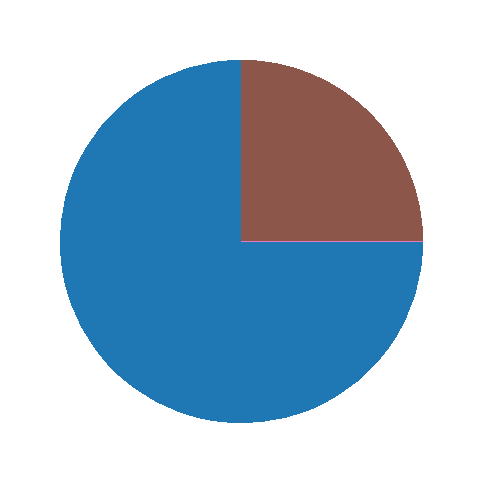
\includegraphics[height=1in]{img/T5}} \\
	\subfigure[][]{
		\label{fig:t6}
		\includegraphics[height=1in]{img/T6}}
	\subfigure[][]{
		\label{fig:t7}
		\includegraphics[height=1in]{img/T7}}
	\subfigure[][]{
		\label{fig:t8}
		\includegraphics[height=1in]{img/T8}}
	\subfigure[][]{
		\label{fig:t9}
		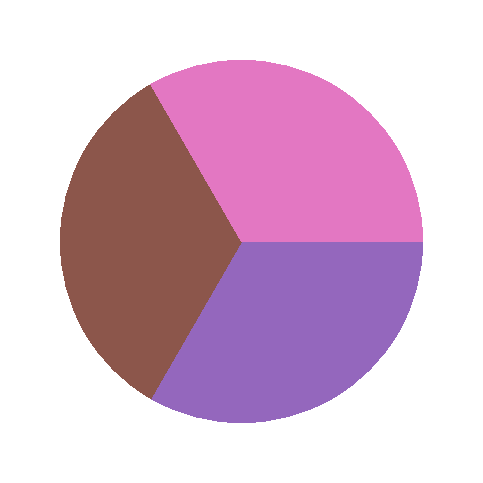
\includegraphics[height=1in]{img/T9}}
	\subfigure[][]{
		\label{fig:t10}
		\includegraphics[height=1in]{img/T10}}
	\caption[Layer distribution of pattern solutions for OWASP top ten]{Layer distribution of security patterns that address the OWASP top ten with one pie chart per vulnerability: 
		\subref{fig:t1} T1;
		\subref{fig:t2} T2;
		\subref{fig:t3} T3; 
		\subref{fig:t4} T4; 
		\subref{fig:t5} T5; 
		\subref{fig:t6} T6; 
		\subref{fig:t7} T7;
		\subref{fig:t8} T8;  
		\subref{fig:t9} T9; and
		\subref{fig:t10} T10.}
	\label{fig:pies}
\end{figure}

Therefore, we see a connection between the found IoT security patterns for a specific OWASP vulnerability and the number of layers the various solutions are from. This assumption is confirmed by the following Figure~\ref{fig:corr}, which consists of a scatter plot that showcases the correlation between the pattern quantity and their layer distribution with a value of 0.86808368. This correlation coefficient always ranges from -1 to 1 and indicates the strength of the relationship between two variables. A value between 0.7 and 1 shows a strong connection and the positive sign indicates, that more patterns as solutions for a specific vulnerability also mean a more diverse distribution of WFRM layers for these IoT patterns. 

\begin{figure}[ht]
	\centering
	\includegraphics[width=0.9\linewidth]{img/correlation}
	\caption{The correlation between the number of patterns and WFRM layers for each OWASP vulnerability.}
	\label{fig:corr}
\end{figure}


\section{Use Case Application}\label{sec:use_case}
Before we discuss the findings of our research work, let's see how the created pattern catalogue can be used in a real life situation. The pattern collection was designed to easily function as a checklist. To showcase the pattern selection process, we describe the following IoT home scenario. It is important to note, that in this example we assume that the system is only used by the owner of the house and no further security measures were taken than the ones that were already integrated into the system. 

This smart home contains different connected devices that are distributed in the living room, bedroom, kitchen, bathroom and entrance of the house. All electronic devices run on the custom firmware Tasmota\footnote{\href{https://tasmota.github.io/docs}{https://tasmota.github.io/docs, last accessed: 25.02.2023.}} and include: Four RGB LED  bulbs\footnote{\href{https://www.tasmota.shop/gb/lights/7-led-rgb-bulb-wifi-e27-15w.html}{https://www.tasmota.shop/gb/lights/7-led-rgb-bulb-wifi-e27-15w.html, last accessed: 25.02.2023.}}, six Shelly\footnote{\href{https://www.shelly.cloud/en-de/products/product-overview/1xs1}{https://www.shelly.cloud/en-de/products/product-overview/1xs1, last accessed: 25.02.2023.}} that function as light controllers, and five smart plugs\footnote{\href{https://www.amazon.de/dp/B07D73S72W}{https://www.amazon.de/dp/B07D73S72W, last accessed: 25.02.2023.}}. In addition, a Raspberry PI with HomeBridge\footnote{\href{https://homebridge.io}{https://homebridge.io, last accessed: 25.02.2023.}} allows the integration of HomeKit into the network that controls the following devices: Two televisions\footnote{\href{https://plugins.hoobs.org/plugin/homebridge-samsung-tizen}{https://plugins.hoobs.org/plugin/homebridge-samsung-tizen, last accessed: 25.02.2023.}}, four Sonos ZonePlayers\footnote{\href{https://plugins.hoobs.org/plugin/homebridge-zp}{https://plugins.hoobs.org/plugin/homebridge-zp, last accessed: 25.02.2023.}}, a Ring camera and doorbell\footnote{\href{https://plugins.hoobs.org/plugin/homebridge-ring}{https://plugins.hoobs.org/plugin/homebridge-ring, last accessed: 25.02.2023.}}.

After we established the use case example, we can inspect each pattern of the catalogue in Chapter~\ref{ch:catalogue} and check its applicability in the given context. The evaluation results can be found in Table~\ref{tab:use-case} with (-) indicating this pattern is not suitable for this system, (o) being used in cases where the given system has already implemented similar security features this pattern would provide, and (+) marking recommended patterns to implement to further optimize the system design.  

\begin{landscape}
\begin{longtable}[c]{llcp{12cm}}
	\caption{Use case applicability of patterns}
	\label{tab:use-case} \\
	\hline
	\textbf{\#} & \textbf{Pattern} & \textbf{Rating} &
	\textbf{Explanation} \\
	\hline
	\endhead
	%
	\ref{p:hardware} & Hardware IoT Security & + & Exchangeable cryptographic co-processors to secure IoT devices. \\
	\ref{p:thing} & Secure IoT Thing & + & Secure any entity that is connected to sensors/actuators, e.g Raspberry PI. \\
	\ref{p:node} & Secure Sensor Node & - & System does not include sensor nodes. \\
	\ref{p:segment} & Security Segmentation & + & IoT devices are divided into subnetworks. \\
	\ref{p:tpm} & Trusted Platform Module & + & Attestation of Raspberry PI with integrated cryptographic services. \\
	\hline
	\ref{p:ac} & Authenticated Channel & o & Mutual authentication of communication partners and forward secrecy. \\
	\ref{p:ec} & Encrypted Channel & o & TLS handshake and exchange of cryptographic information. \\
	\ref{p:broker} & Middleware Message Broker & o & HomeBridge controls the flow of messages between IoT devices. \\
	\ref{p:scmessage} & Middleware Self-contained Message & + & Messages should be \q{pure and complete} representations of events/commands. \\
	\ref{p:sdn} & Orchestration of SDN Network Elements & - & Only required when an IoT SDN is employed. \\
	\ref{p:con} & Outbound-Only Connection & + & Blocks incoming malicious connection requests. \\
	\ref{p:keyex} & Password Based Key Exchange & + & Common secret is used to generate session key pairs. \\
	\ref{p:sc} & Safe Channel & o & Use certificates to guarantee integrity during message transmission. \\
	\ref{p:readout} & Secure Remote Readout & + & Security Module encrypts measurements before transmitting. \\
	\ref{p:sm} & Signed Message & o & Use digital signatures during the message generation/exchange process. \\
	\ref{p:crypto} & Symmetric Key Cryptography & + & Handshake and common secret are exchanged between communication parties. \\
	\ref{p:auc} & Third Party Based Authentication & + & Combination of asymmetric cryptography and session keys. \\
	\ref{p:partner} & Trusted Communication Partner & + & List trusted communication partners and block unknown connection requests. \\
	\ref{p:trust} & Web of Trust & - & Tasmota uses a central self-signed certificate authority. \\
	\hline
	\ref{p:fog} & Fog Computing & - & No cloud-based system. \\
	\ref{p:fogxy} & Fogxy & - & No cloud-based system. \\
	\ref{p:cloud} & Secure Cloud-based IoT Architecture & - & No cloud-based system. \\
	\hline
	\ref{p:es} & Encrypted Storage & + & Critical data is encrypted before it gets committed to disk. \\
	\ref{p:rs} & Redundant Storage & - & No cloud-based system. \\
	\ref{p:ss} & Safe Storage & + & Guarantee integrity of stored data. \\
	\hline
	\ref{p:translation} & Alignment-based Translation Pattern & o & HomeBridge enables interoperability between different platforms. \\
	\ref{p:block} & BlockBD & - & No Big Data system. \\
	\ref{p:discover} & Discovery of IoT Services & - & No usage of different IoT services. \\
	\ref{p:flow} & Flow-based Service Composition & - & No usage of different IoT services. \\
	\ref{p:gateway} & IoT Gateway Event Subscription & o & HomeBridge sends notifications on updates. \\
	\hline
	\ref{p:ssl} & IoT SSL Cross-Layer Secure Access & o & Only authenticated entities are able to access the external interfaces. \\
	\ref{p:msgtranslator} & Middleware Message Translator & o & HomeBridge enables interoperability between different platforms. \\
	\ref{p:middleware} & Middleware Simple Component & + & Universally applicable pattern to achieve the best component decomposition. \\
	\ref{p:rest} & REST Request/Response & o & HomeBridge API is used to connect to different IoT devices. \\
	\ref{p:sandbox} & Server Sandbox & + & Isolate server to protect it in case the system gets compromised. \\
	\ref{p:orchest} & Service Orchestration & - & No usage of different IoT services. \\
	\ref{p:ontology} & Translation with Central Ontology & o & HomeBridge enables interoperability between different platforms. \\
	\hline
	\ref{p:acp} & Access Control to Physical Structures & - & No physical structures need to be accessed. \\
	\ref{p:alarm} & Alarm Monitoring & o & Alarm functionality is included in HomeBridge. \\
	\ref{p:log} & Audit Log & o & HomeBridge has a rolling log screen. \\
	\ref{p:acs} & Authenticated Session & - & System runs on a local server with no internet requirements. \\
	\ref{p:aze} & Authorization Enforcer & - & Only relevant if system is used by users with different roles. \\
	\ref{p:ep} & Encrypted Processing & + & Integrity of data with e.g homomorphic functions or secure multi-party computation. \\
	\ref{p:fault} & Fault Management & + & Smart handling of any faulty behaviour of the system. \\
	\ref{p:fac} & File Authentication & - & Only relevant if system is used by users with different privileges. \\
	\ref{p:mac} & Matrix Authentication & - & Only relevant if system is used by users with different privileges. \\	
	\ref{p:mine} & Minefield & + & Modify Raspberry PI to confuse attackers and simplify threat detection. \\
	\ref{p:rac} & Remote Authenticator/Authorizer & - & System runs on a local server with no internet requirements. \\
	\ref{p:rbac} & Role Based Access Control & - & Only relevant if system is used by users with different roles. \\
	\ref{p:sp} & Safe Processing & + & Guarantee integrity during data processing with e.g integrity checks. \\
	\ref{p:sdps} & Secure Distributed Publish/Subscribe & o & HomeBridge sends notifications on updates. \\
	\ref{p:uptime} & Uptime & o & HomeBridge measures and displays the server availability. \\
	\hline
	\ref{p:lockout} & Account Lockout & o & Login via password authentication. \\
	\ref{p:ace} & Authentication Enforcer & + & Authentication process that creates a proof of identity. \\
	\ref{p:black} & Blacklist & + & Identification of abusers who are not granted access to the system. \\
	\ref{p:hauc} & History-Based Authentication & + & Authentication is based on the user's own history. \\	
	\ref{p:control} & Permission Control & + & User can control which data is shared with the server. \\
	\ref{p:hub} & Personal Zone Hub & - & No cloud-based system. \\
	\ref{p:relays} & Relays & - & No switches in the system. \\
	\hline
	\ref{p:sap} & Single Access Point & + & Only one entry point into the system with HomeBridge UI. \\
	\ref{p:white} & Whitelist & + & Identification of trusted communication partners. \\
	\hline
\end{longtable}
\end{landscape}

While there are many patterns that are not suitable to be implemented in this kind of smart home scenario, like BlockBD~\ref{p:block} or the Web of Trust~\ref{p:trust}, just as many are already integrated into the system, e.g Uptime~\ref{p:uptime} or Account Lockout~\ref{p:lockout}. Nevertheless by going through the catalogue and analysing each pattern individually, we found 25 patterns that can be used to optimize the security measures in this smart home example. Spread across all layers of the WFRM architecture, one can choose from a variety of patterns that include Symmetric Key Cryptography~\ref{p:hardware}, Server Sandbox~\ref{p:sandbox} or even simpler solutions like a combination of a Blacklist~\ref{p:black} and a Whitelist~\ref{p:white}. 

This use case demonstrates that our pattern catalogue can act as an easy guideline to improve the security of a system. The evaluation process can be as straightforward as using the catalogue as a checklist while other approaches could include the sorting by WFRM layers or even by security objectives. Regardless of which method one uses, every system has vulnerabilities that can benefit from even the most obvious or trivial security features, like a Single Access Point~\ref{p:sap}.



 


% !TeX encoding = UTF-8
% !TeX spellcheck = en_GB
% !TeX root = ../thesis.tex

\chapter{Discussion}\label{ch:discussion}
In this last chapter we point out the threats to validity of our research work (see Section~\ref{sec:threats}) as well as suggest areas in the IoT security field that need more investigation in the future in Section~\ref{sec:future_work}. Lastly a final conclusion to close off this master's thesis is given in Section~\ref{sec:conclusion}.

\section{Threats to Validity}\label{sec:threats}
Like for any type of research work, there exist specific limitations that must be considered when looking at the context of a dissertation. Internal as well as external factors that cannot be influenced by the researcher can lessen the validity of the analysis and its conclusions. These threats also exist in this master's thesis and can be listed as the following points:

\paragraph{Lacking Data Set.} The process of automated and manual searching, collecting and scanning publications that fit into the theme of this master's thesis can be quite challenging. We have to decide which patterns have a focus on IoT security and are truly pieces of a solution to a larger problem and not entire architectures by themselves. Therefore the creation of a complete and structured pattern catalogue from scratch is an impossible task and prone to errors and missing patterns.

\paragraph{Indefinite Categorizations.} Defining different patterns and putting them into specific categories can be a difficult task. When assigning these patterns to the different layers of the IoT WFRM, we did it with the best of our ability. But these categories can be interpreted in different ways and a pattern can be attributed to more than one layer. So there are many possibilities on where to draw the lines. 

\paragraph{Outdated OWASP Top Ten.} To have an up-to-date discussion on the topic of IoT security patterns, we tried to take the newest research into account in our analysis. But this is not always possible. In the case of the referenced OWASP top ten list on the common IoT vulnerabilities, the ranking was last updated in 2018. So the possibility that the rankings have changed in the last couple of years is huge because of how fast technology evolves these days. This has to be taken into consideration, when we analyse how these vulnerabilities can be solved with our pattern catalogue and which risks still exist in IoT systems today.


\section{Future Work}\label{sec:future_work}
A collection of security patterns in the IoT field is a good start to get an overview of the current state of the art. But there are many more ways in which researchers and developers can advance the secure IoT development and utilize the advantages of standardization.  

\paragraph{\textbf{Pattern Catalogue Expansion.}} The IoT security pattern catalogue in Chapter~\ref{ch:catalogue} cannot be called complete in any way. There are surely more security patterns that can be modified into the IoT context as well as other types of patterns that can make the implementation of secure IoT systems easier. A few examples would be privacy patterns, misuse patterns or anti-patterns. Therefore, the expansion of the security pattern catalogue for IoT is definitely a topic for further research.   

\paragraph{\textbf{Industry Cooperation.}} Technology and science are ever-evolving, therefore the need for different types of patterns for common problems will always exist and require new and modern solutions. The best way to develop new security patterns, that are optimized for applicability and usage in real-world situations, is a cooperation with the industry. Only when academia combines its theories and ideas with the practical problems of the corresponding industry, we will find the best solutions to solve common issues in the world of IoT. 

\paragraph{\textbf{IoT Security Architectures.}} The last point would be the usage of existing security patterns to model architectures that are able to protect IoT systems from cyberattacks. By combining specific security patterns we will be able to create improved IoT systems in the future. 


\section{Conclusion}\label{sec:conclusion}
The aim of this analysis was to identify the shortcomings of the state-of-the-art research in the field of IoT security and to provide a guide for future development of secure IoT systems. 

In the beginning we defined, which IoT devices belong into the IoT spectrum and in which areas of life these are found. Regardless if you look into the healthcare, banking or industry sector, IoT applications exist everywhere they can be useful. Even a small home can benefit from the safety features of IoT gadgets like motion detectors, security cameras or smart locks.

After gaining a better understanding of the topic, we further inspected various threats in the IoT field that can be caused by cyberattacks and harm the safety of its users. Attackers can infiltrate a system by using techniques like man-in-the-middle, denial of service or even ransomware. In addition, we looked at a list of IoT vulnerabilities, such as unsecure passwords or system components, and how to overcome these threats by utilizing secure-by-design architecture.  

After introducing the IoT WFRM and an overview of the most important security objectives, our goal was to create a comprehensive catalogue of IoT security patterns. Although one can never say such a collection is complete, the catalogue includes all findings we could make under the given search criteria. Furthermore, these patterns allowed us to gain knowledge about the following questions:

\begin{itemize}
	\item Which layer in the IoT WFRM is covered by the least security patterns?
	\item Which security goal is addressed by security patterns the least and how can the coverage be improved?
	\item How many of the OWASP top ten most common IoT vulnerabilities are solved by utilizing these security patterns?
\end{itemize}

With a catalogue that consists of 61 patterns, it was surprising that almost half of these belonged to only two layers. Also, the lack of security goals that were covered in the Data Accumulation layer is alarming. On the other hand every vulnerability, that was published by OWASP, was addressed by at least one pattern, which is a positive discovery. 

To sum up, with these findings we built a foundation for future endeavours to broaden the spectrum of IoT security patterns. Thus, this pattern catalogue can be used as a starting point for secure system design or further academic research, that will expand the current number of entries in our pattern collection. With appropriate industry cooperation the development of applicable patterns, that improve the security of IoT systems and at the same time protect its users, can be achieved.



%\appendix
%% !TeX spellcheck = en_GB
% !TeX encoding = UTF-8
% !TeX root = ../thesis.tex
\chapter{Code}

\chapter{Math}

\chapter{Dataset}



\listoffigures
\listoftables



% References (Literaturverzeichnis):
% a) Style (with numbers: use unsrt):
\bibliographystyle{alpha}
% b) The File:
\bibliography{Bibliography}


%%%%%%%%%%%%%%%%%%%%%%%%%%%%%%%%%%%%%%%%%%%%%%%%%%%%%%%%%%%%


%%%%%%%%%%%%%%%%%%%%%%%%%%%%%%%%%%%%%%%%%%%%%%%%%%%%%%%%%%%%


%%%%%%%%%%%%%%%%%%%%%%%%%%%%%%%%%%%%%%%%%%%%%%%%%%%%%%%%%%%%
\end{document}
